\documentclass[information,article,submit,moreauthors,pdftex]{Definitions/mdpi} 

\firstpage{1} 
\makeatletter 
\setcounter{page}{\@firstpage} 
\makeatother
\pubvolume{1}
\issuenum{1}
\articlenumber{0}
\pubyear{2021}
\copyrightyear{2021}
\datereceived{} 
\dateaccepted{} 
\datepublished{} 
\hreflink{https://doi.org/}

\usepackage{breakcites}
\usepackage{float}
\usepackage{graphicx}
\usepackage{subcaption}
\usepackage{geometry}
\usepackage{amsmath}
\newcommand{\inlineeqnum}{\refstepcounter{equation}~~\mbox{(\theequation)}}
\usepackage{enumitem}
\usepackage[ruled,vlined]{algorithm2e}
\usepackage{booktabs}
\usepackage{pgfplotstable}
\pgfplotsset{compat=1.17}
\usepackage{longtable}
\usepackage{tabu}
\usepackage{hyperref}

% Used to track changes. Can be deleted once the revision process is over.
% commands:
% \added
% \deleted
% \replaced
\usepackage{changes}

\makeatletter
\@namedef{Changes@AuthorColor}{red}
\colorlet{Changes@Color}{red}
\makeatother

\Title{Improving Imbalanced Land Cover Classification with K-means SMOTE:
Detecting and Oversampling Distinctive Minority Spectral Signatures}

% MDPI internal command: Title for citation in the left column
\TitleCitation{Improving Imbalanced Land Cover Classification with K-means SMOTE:
Detecting and Oversampling Distinctive Minority Spectral Signatures}

% Orcid ID
\newcommand{\orcidauthorA}{0000-0001-5889-3575}
\newcommand{\orcidauthorB}{0000-0001-7019-3782}
\newcommand{\orcidauthorC}{0000-0002-0834-0275}

\Author{
    Joao Fonseca $^{1,}$*\orcidA{},
    Georgios Douzas $^{1}$\orcidB{},
    Fernando Bacao $^{1}$\orcidC{}
}

% MDPI internal command: Authors, for metadata in PDF
\AuthorNames{Joao Fonseca, Georgios Douzas and Fernando Bacao}

% MDPI internal command: Authors, for citation in the left column
\AuthorCitation{Fonseca, J.; Douzas, G.; Bacao, F.}

\address{%
$^{1}$ \quad NOVA Information Management School (NOVA IMS), Universidade Nova
    de Lisboa, Campus de Campolide, 1070-312 Lisboa, Portugal;
    gdouzas@novaims.unl.pt (G.D.); bacao@novaims.unl.pt (F.B.)\\
    * \quad Correspondence: jpfonseca@novaims.unl.pt (J.F.)
}

\corres{Correspondence: jpfonseca@novaims.unl.pt}


\abstract{
    Land cover maps are a critical tool to support informed policy
    development, planning, and resource management decisions. \deleted{The
    ability to automatically produce Land Use/Land Cover (LULC) maps, through
    the use of machine learning methods, will improve the accuracy and
    timeliness of decision-making.} With significant upsides, the automatic
    production of Land Use/Land Cover maps has been a topic of interest for
    the remote sensing community for several years, but it is still fraught
    with technical challenges. One such challenge is the imbalanced nature of
    most remotely sensed data\deleted{, where the number of samples of a few
    classes is significantly greater than the number of samples of the
    remaining classes}. \replaced{The}{This} asymmetric class distribution
    impacts negatively the performance of classifiers and adds a new source of
    error to the production of these maps. In this paper, we address the
    imbalanced learning problem, by using K-means and the Synthetic Minority
    Oversampling TEchnique (SMOTE) as an improved oversampling algorithm.
    K-Means SMOTE improves the quality of newly created artificial data by
    addressing both the between-class imbalance, as traditional oversamplers
    do, but also the within-class imbalance, avoiding the generation of noisy
    data while effectively overcoming data imbalance. The performance of
    K-means SMOTE is compared to \added{three} popular oversampling methods
    \added{(Random Oversampling, SMOTE and Borderline-SMOTE)} using seven
    remote sensing benchmark datasets, three classifiers \added{(Logistic
    Regression, K-Nearest Neighbors and Random Forest Classifier)} and
    \added{three} evaluation metrics \added{using a 5-fold cross-validation
    approach with 3 different initialization seeds}. The statistical analysis
    of the results show that the proposed method consistently outperforms the
    remaining oversamplers producing higher quality land cover
    classifications. These results suggest that LULC data can benefit
    significantly from the use of more sophisticated oversamplers as spectral
    signatures for the same class can vary according to geographical
    distribution.
}

\keyword{
    LULC Classification; 
    Imbalanced Learning; 
    Oversampling; 
    Data Augmentation; 
    Clustering
} 

\begin{document}

\section{Introduction}

The increasing amount of remote sensing missions granted the access to dense
time series (TS) data at a global level and provides up-to-date, accurate land
cover information \citep{Drusch2012}. This information is often materialized
through Land Use and Land Cover (LULC) maps. While Land Cover maps
define the biophysical cover found on the surface of the earth, Land Use maps
define how it is used by humans \citep{Fritz2017}. Both Land Use and Land Cover
maps constitute an essential asset for various purposes, such as land cover
change detection, urban planning, environmental monitoring and natural hazard
assessment \citep{Khatami2016}. However, the timely production of accurate and
updated LULC maps is still a challenge within the remote sensing community
\citep{Wulder2018}. LULC maps are produced based on two main approaches:
photo-interpreted by the human eye, or automatic mapping using remotely sensed
data and classification algorithms.

While photo-interpreted LULC maps rely on human operators and can be more
reliable, they also present some significant disadvantages. The most important
disadvantage is the cost of production, in fact photo-interpretation consumes
significant resources, both in terms of money and time. Because of that, they
are not frequently updated and not suitable for operational mapping over large
areas.  Finally, there is also the issue of overlooking rare or small-area
classes, due to factors such as the minimum mapping unit being used.

Automatic mapping with classification algorithms based on machine-learning
(ML) have been extensively researched and used to speed up and reduce the
costs of the production process \citep{Khatami2016, Gavade2019,
Kaur2019}. Improvements in classification algorithms are sure to have
significant impact in the efficiency with which remote sensing imagery is
used. Several challenges have been identified in order to improve automatic
classification:

\begin{enumerate}
    \item Improve the ability to handle high-dimensional datasets, in cases
        such as Multi-spectral TS composites high-dimensionality increases the
        complexity of the problem and creates a strain on computational power
        \citep{Stromann2020}.
    \item Improve class separability, as the production of an accurate LULC map
        can be hindered by the existence of classes with similar spectral
        signatures, making these classes difficult to distinguish
        \citep{Alonso-Sarria2019}.
    \item Resilience to mislabelled LULC patches, as the use of
        photo-interpreted training data poses a threat to the quality of any
        LULC map produced with this strategy, since factors such as the minimum
        mapping unit tend to cause the overlooking of small-area LULC patches
        and generates noisy training data that may reduce the prediction
        accuracy of a classifier \citep{Pelletier2017}.
    \item Dealing with rare land cover classes, due to the varying levels of
        area coverage for each class. In this case using a purely random
        sampling strategy will amount to a dataset with a roughly proportional
        class distribution as the one on the multi/hyperspectral
        image. On the other hand, the acquisition of training
        datasets containing balanced class frequencies is often unfeasible.
        This causes an asymmetry in class distribution, where some classes are
        frequent in the training dataset, while others have little expression
        \citep{Wang2019, Feng2019}.
\end{enumerate}

The latter challenge is known, in machine learning, as the imbalanced learning
problem \citep{Chawla2004}. It is defined as a skewed distribution of instances
found in a dataset among classes in both binary and multi-class problems
\citep{Abdi2016}. This asymmetry in class distribution negatively impacts the
performance of classifiers, especially in multi-class problems.  The problem
comes from the fact that during the learning phase, classifiers are optimized
to maximize an objective function, with overall accuracy being the most common
one \citep{Maxwell2018}. This means that instances belonging to minority
classes contribute less to the optimization process, translating into a bias
towards majority classes. As an example, a trivial classifier can achieve 99\%
overall accuracy on a binary dataset where 1\% of the instances belong to the
minority class if it classifies all instances as belonging to the majority
class. This is an especially significant issue in the automatic classification
of LULC maps, as the distribution of the different land-use classes tends to
be highly imbalanced.  Therefore, improvements in the ability to deal with
imbalanced datasets will translate into important progress in the automatic
classification of LULC maps.

There are three different types of approaches to deal with the class imbalance
problem \citep{Fernandez2013,Kaur2019}:

\begin{enumerate}
    \item Cost-sensitive solutions. Introduces a cost matrix to the learning
        phase with misclassification costs attributed to each class. Minority
        classes will have a higher cost than majority classes, forcing the
        algorithm to be more flexible and adapt better to predict minority
        classes.
    \item Algorithmic level solutions. Specific classifiers are modified to
        reinforce the learning on minority classes. Consists on the creation or
        adaptation of classifiers.
    \item Resampling solutions. Rebalances the dataset's class distribution by
        removing majority class instances and/or generating artificial minority
        instances. This can be seen as an external approach, where the
        intervention occurs before the learning phase, benefitting from
        versatility and independency from the classifier used.
\end{enumerate}

Since resampling strategies represent a set of methods that are detached from
classifiers by operating at the data level, they allow the use of any off the
shelf algorithm, without the need for any type of changes or adaptions to the
algorithm. Specifically, in the case of oversampling (defined below), the user
is able to balance the dataset's class distribution by without the loss of
information, which is not the case with undersampling techniques. This is a
significant advantage especially considering that most users in remote sensing
are not expert machine learning engineers. 

Within resampling approaches there are three subgroups of approaches
\citep{Fernandez2013,Kaur2019,Luengo2020}:

\begin{enumerate}
    \item Undersampling methods, which rebalance class distribution by removing
        instances from the majority classes.
    \item Oversampling methods, which rebalance datasets by generating new
        artificial instances belonging to the minority classes.
    \item Hybrid methods, which are a combination of both oversampling and
        undersampling, resulting in the removal of instances in the majority
        classes and the generation of artificial instances in the minority
        classes.
\end{enumerate}

Resampling methods can be further distinguished between non-informed and
heuristic (i.e., informed) resampling techniques
\citep{Fernandez2013,Luengo2020,Garcia2016}. The former consist of methods that
duplicate/remove a random selection of data points to set class distributions
to user-specified levels, and are therefore a simpler approach to the problem.
The latter consists of more sophisticated approaches that aim to perform
over/undersampling based on the points' contextual information within their
data space.

The imbalanced learning problem is not new in machine learning but its
relevancy has been growing, as attested by \citep{Haixiang2017}. The problem
has also been addressed in the context of remote sensing \citep{Douzas2019rs}.
In this paper, we propose the application of a recent oversampler based
on SMOTE \citep{Chawla2002}, the K-means SMOTE 
\citep{Douzas2018} oversampler, to address the imbalanced learning
problem in a multiclass context for LULC classification using various remote
sensing datasets. Specifically, we use seven land use datasets commonly
used in research literature, that vary among agricultural and urban land use.
The K-means SMOTE algorithm couples two different
procedures in the generation of artificial data. The algorithm starts by
grouping the instances into clusters by using the K-means
algorithm; next, the generation of the artificial
data is done using the smote algorithm, taking into consideration the distribution of
majority/minority cases in each individual cluster. The idea of starting with
a clustering procedure before the data generation phase is important in remote
sensing because the spectral signature of the different classes can change
significantly based on the geographical area in which it is represented. In
other words, the spectral signature of a specific class can vary greatly
depending on the geography, meaning that often we will be facing within-class
imbalance \citep{Japkowicz2001}.

In fact, we can decompose class imbalance into two different types:
between-class imbalance and within-class imbalance \citep{Douzas2018, Jo2004}.
While the first refers to the overall asymmetry between majority and minority
classes, the second results from the fact that in different areas of the input
space there might be different levels of imbalance. Depending on the
complexity of the input space, different subclusters of minority and majority
instances may be present. In order to achieve a balance between minority and
majority instances, these subclusters should be treated separately. Assuming
that the role of a classifier is to create rules in such a way that it is able
to isolate the different relevant sub-concepts that represent both the
majority and minority classes, the classifier will create multiple disjunct
rules that describe these concepts. If the input space is simple and the
classes’ instances are grouped together in a unique cluster, the classifier
will only need to create (general) rules that comprise large portions of
instances belonging to the same class. To the contrary, if the input space is
complex and scatters through multiple small clusters, the classifier will need
to learn a more complex set of (specific) rules, which can be seen in Figure
\ref{fig:complex_input_space_example}. It is important to note that small
clusters can happen both in the minority and majority class, although they
will tend to be more frequent in the minority class due to its
underrepresentation.  

\end{paracol}
\begin{figure}[ht]
    \widefigure
    \captionsetup{justification=centering}
	\caption{Example of a complex input space. In this example, a classifier
        would need to separate the minority class' samples across 4
        distinguishable clusters (A, B, C and D).
    \vspace{.2cm}}
	\label{fig:complex_input_space_example}
	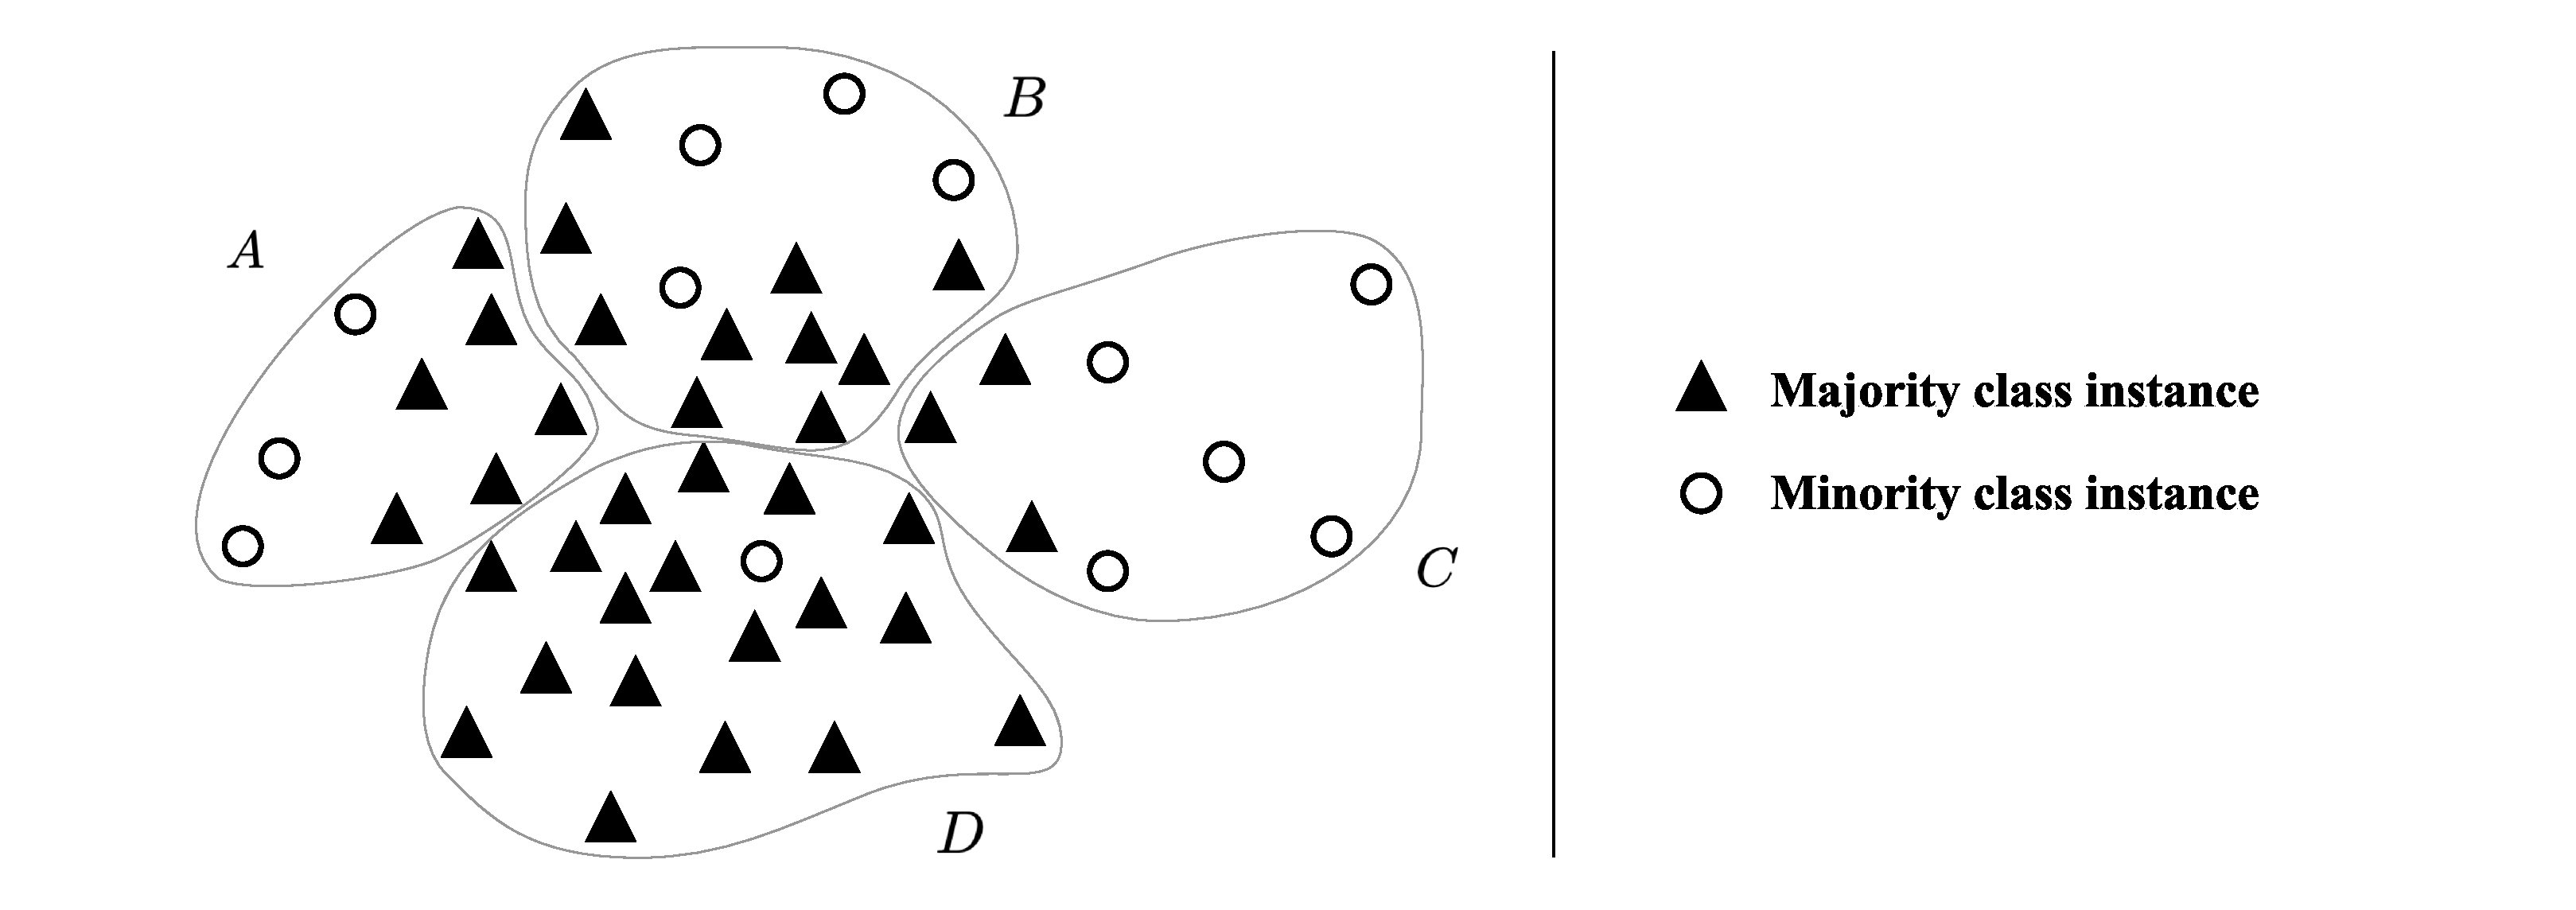
\includegraphics[width=1\linewidth]{../analysis/complex_input_space_example}
\end{figure}
\begin{paracol}{2}
\linenumbers
\switchcolumn

The efficacy of K-means SMOTE is tested using different
types of classifiers. To do so, we employ both commonly used and/or
state-of-the-art oversamplers as benchmarking methods: Random oversampling
(ROS), SMOTE and Borderline-SMOTE (B-SMOTE) \citep{Han2005}. Also
as a baseline score we include classification results without the use of any
resampling method.

This paper is organized in 5 sections: section \ref{sec:sota} provides an
overview of the state-of-art, section \ref{sec:methodology} describes the
proposed methodology, section \ref{sec:results} covers the results and
discussion and section \ref{sec:conclusion} presents the conclusions taken from
this study.

This paper's main contributions are:
\begin{itemize}
    \item Propose a cluster-based multiclass oversampling method appropriate
        for LULC classification and compare its performance with the remaining
        oversamplers in a multiclass context with seven benchmark LULC
        classification datasets. Allows us to check the oversamplers'
        performance across benchmark LULC datasets.
    \item Introducing a cluster-based oversampling algorithm within the remote
        sensing domain, as well as comparing its performance with the remaining
        oversamplers in a multiclass context.
    \item Make available to the remote sensing community the implementation
        of the algorithm in a Python library and the experiment's source
        code.
\end{itemize}

\section{Imbalanced Learning Approaches} \label{sec:sota}

Imbalanced learning has been addressed in three different ways:
over/undersampling, cost-sensitive training and changes/adaptations in the
learning algorithms \citep{Kaur2019}. These approaches impact different
phases of the learning process, while over/undersampling can be seen as a
pre-processing step, cost-sensitive and changes in the algorithm imply a more
customized and complex intervention in the algorithms. In this
section, we focus on previous work related with resampling methods, while
providing a brief explanation of cost-sensitive and algorithmic level solutions.

All of the most common classifiers used for LULC classification tasks
\citep{Khatami2016, Gavade2019} are sensitive to class imbalance
\citep{Blagus2010}. Algorithm-based approaches typically focus on adaptations
based on ensemble classification methods \citep{Mellor2015} or common
non-ensemble based classifiers such as Support Vector Machines \citep{Shao2014}.
In \citep{Lee2016}, the reported results show that algorithm-based methods have
comparable performance to resampling methods.

Cost-sensitive solutions refer to changes in the importance attributed to each
instance through a cost matrix \citep{Huang2016,Cui2019,Dong2017}. A
relevant cost sensitive solution
\citep{Huang2016} uses  the inverse class frequency (i.e., $1/|C_i|$, where $C_i$ refers
to the frequency of class $i$) to give higher weight to
minority classes. Cui et al. \citep{Cui2019} extended this method by adding a
hyperparameter $\beta$ to class weights as $(1-\beta)/(1-\beta^{|C_i|})$. When
$\beta=0$, no re-weighting is done. When $\beta\rightarrow 1$, weights are the
inverse of the frequency class matrix. Another method \citep{Dong2017} explores
adaptations of Cross-entropy classification loss by adding different
formulations of class rectification loss.

Resampling (over/undersampling) is the most common approach to imbalanced
learning in machine
learning in general and remote sensing in particular \citep{Feng2019}. The
generation of artificial instances (i.e., augmenting the dataset), based on
rare instances, is done independently of any other step in the learning
process. Once the procedure is applied, any standard machine learning
algorithm can be used. Its simplicity makes resampling strategies particularly
appealing for any user (especially the non-sophisticated user) interested in
applying several classifiers, while maintaining a simple approach. It is also
important to notice that over/undersampling methods can also be easily applied
to multiclass problems, common in LULC classification tasks.

\subsection{Non-informed resampling methods}

There are two main non-informed resampling methods. Random Oversampling (ROS)
generates artificial instances through random duplication of minority class
instances. This method is used in remote sensing for its simplicity
\citep{Sharififar2019, Hounkpatin2018}, even though its mechanism makes the
classifier prone to overfitting \citep{Krawczyk2016}. \cite{Hounkpatin2018}
found that using ROS returned worse results than keeping the original
imbalance in their dataset.

A few of the recent remote sensing studies employed Random Undersampling (RUS)
\citep{Ferreira2019}, which randomly removes instances belonging to majority
classes. Although it's not as prone to overfitting as ROS, it incurs into
information loss by eliminating instances from the majority class
\citep{Feng2019}, which can be detrimental to the quality of the results.

Another disadvantage of non-informed resampling methods is their
performance-wise inconsistency across classifiers. ROS' impact on the Indian
Pines dataset was found inconsistent between Random Forest Classifiers (RFC)
and Support Vector Machines (SVM) and lowered the predictive power of an
artificial neural network (ANN) \citep{Maxwell2018}. Similarly, RUS is found to
generally lead to a lower overall accuracy due to the associated information
loss \citep{Maxwell2018}.

\subsection{Heuristic methods}

The methods presented in this section appear as a means to overcome the
insufficiencies found in non-informed resampling. They use either local or
global information to generate new, relevant, non-duplicated instances to
populate the minority classes and/or remove irrelevant instances from majority
classes. In a comparative analysis between over- and undersamplers' performance
for LULC classification \citep{Feng2018} using the rotation forest ensemble
classifier, authors found that oversampling methods consistently outperform
undersampling methods. This result led us to exclude undersampling from our
study.

SMOTE \citep{Chawla2002} was the first heuristic oversampling algorithm to be
proposed and has been the most popular one since then, likely due to its fair
degree of simplicity and quality of generated data. It takes a random minority
class sample and introduces synthetic instances along the line segment that
join a random $k$ minority class nearest neighbor to the selected sample.
Specifically, a single synthetic sample $\overrightarrow{z}$ is generated
within the line segment of a randomly selected minority class
instance $\overrightarrow{x}$ and one of its $k$ nearest
neighbors $\overrightarrow{y}$ such that $\overrightarrow{z} =
\alpha\overrightarrow{x}+(1-\alpha)\overrightarrow{y}$, where $\alpha$ is a
random real number between 0 and 1, as shown in
Figure \ref{fig:smote_example}.

\end{paracol}
\begin{figure}
	\centering
    \captionsetup{justification=centering}
    \caption{Example of SMOTE's data generation process. SMOTE randomly
        selects instance $\protect\overrightarrow{x}$ and randomly selects one
        of its k-nearest neighbors $\protect\overrightarrow{y}$ to produce
        $\protect\overrightarrow{z}$.  Noisy instance
        $\protect\overrightarrow{r}$ was generated by randomly selecting
        $\protect\overrightarrow{q}$ and randomly selecting its nearest
        neighbor $\protect\overrightarrow{p}$ from a different minority class
        cluster. Noisy instance $\protect\overrightarrow{c}$ was generated by
        randomly selecting the noisy minority class instance
        $\protect\overrightarrow{a}$ and one of its nearest neighbors
        $\protect\overrightarrow{b}$.
    \vspace{.2cm}}
	\label{fig:smote_example}
	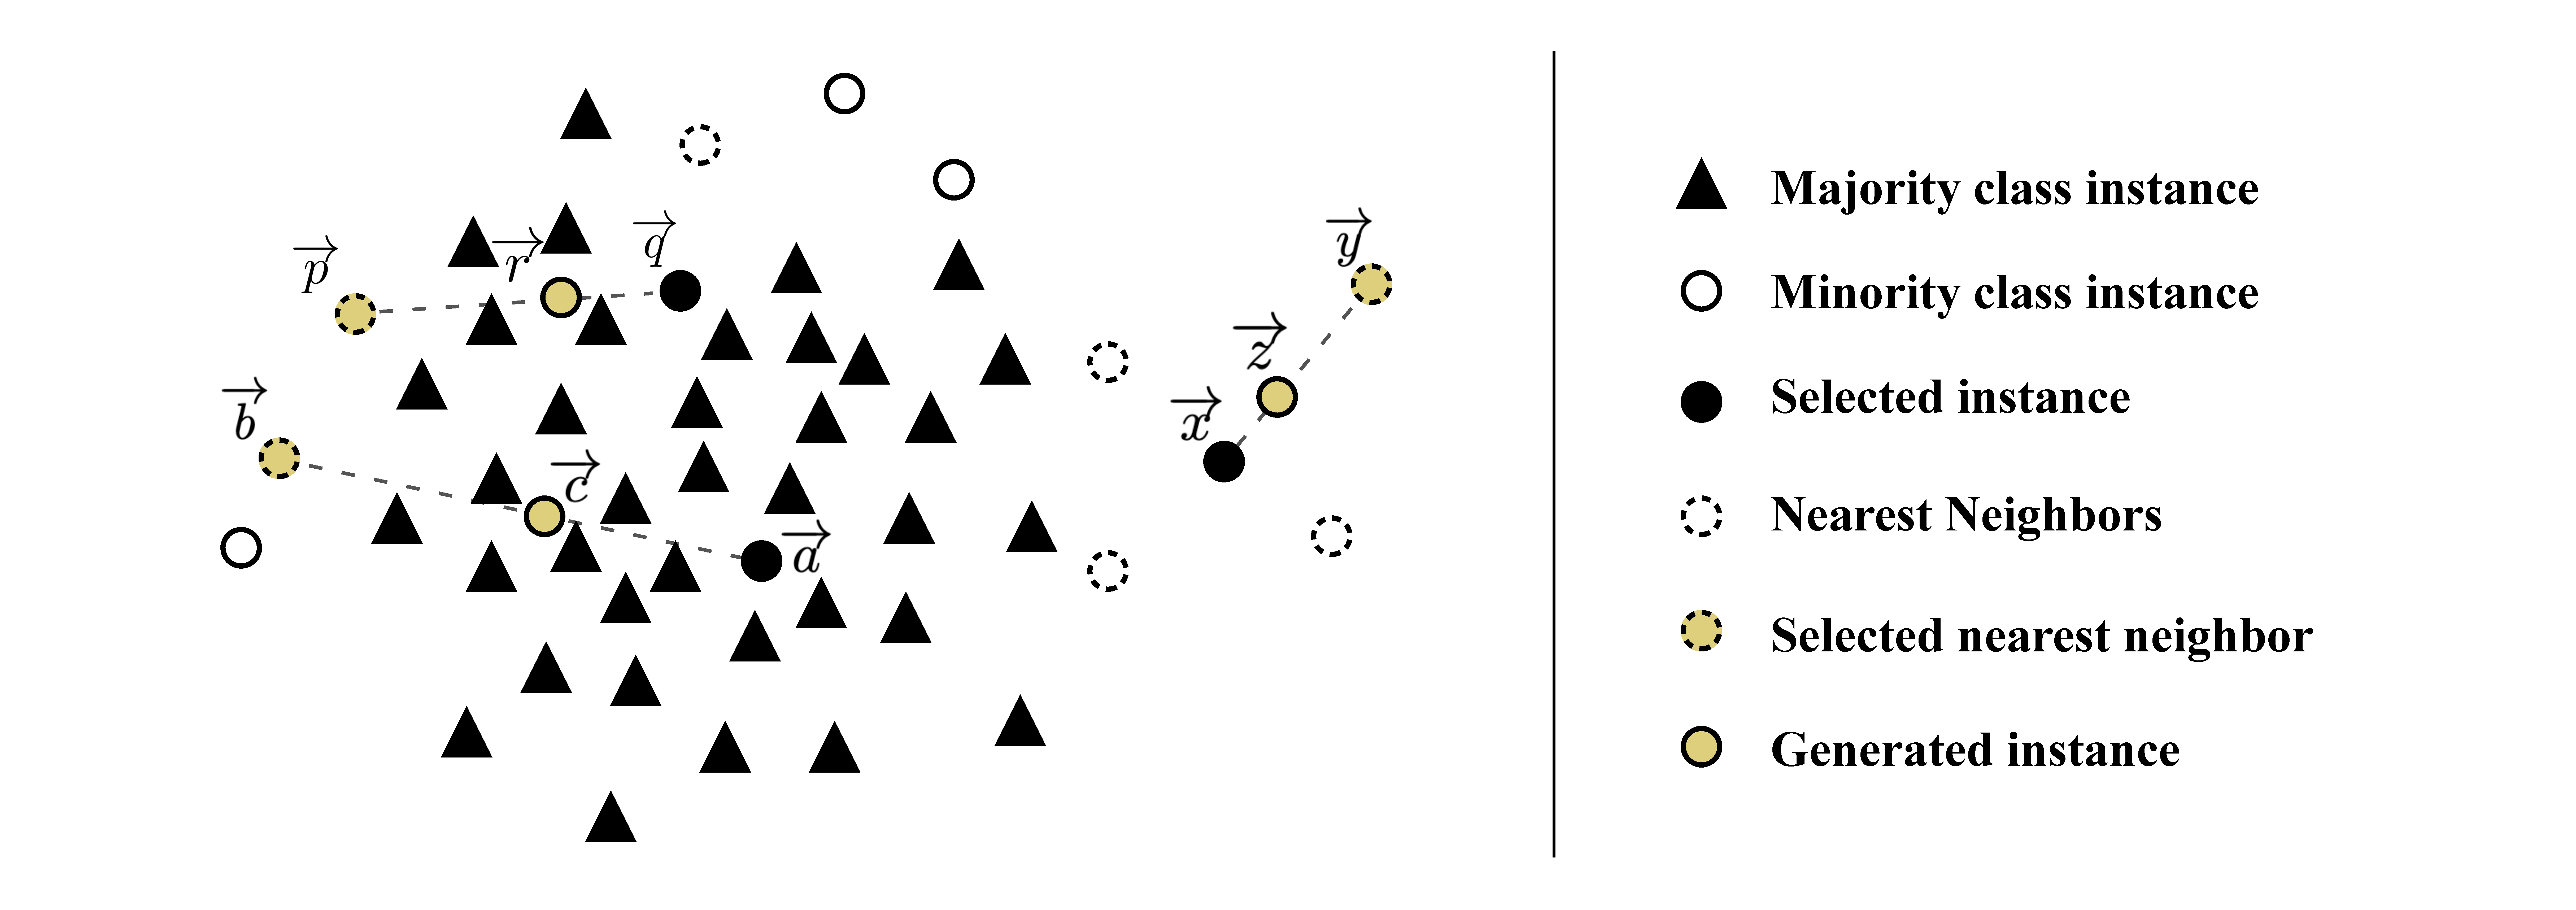
\includegraphics[width=1\linewidth]{../analysis/smote_example}
\end{figure}
\begin{paracol}{2}
\linenumbers
\switchcolumn

A number of studies implement SMOTE within the LULC classification context and
reported improvements on the quality of the trained predictors
\citep{Jozdani2019, Bogner2018}. Another study proposes an adaptation of SMOTE
on an algorithmic level for deep learning applications \citep{Zhu2020}. This
method combines both typical computer vision data augmentation techniques,
such as image rotation, scaling and flipping on the generated instances to
populate minority classes. Another algorithmic implementation is the
variational semi-supervised learning model \citep{Cenggoro2018}. It consists of
a generative model that allows learning from both labeled and unlabeled
instances while using SMOTE to balance the data.

Despite SMOTE's popularity, its limitations have motivated the development of
more sophisticated oversampling algorithms \citep{Douzas2019, Han2005, Ma2017,
Douzas2017, Douzas2018, HaiboHe2008}. \cite{Douzas2019} identify four major
weaknesses of the SMOTE algorithm, which can be summarized as:

\begin{enumerate}
    \item Generation of noisy instances due to random selection of a
        minority instance to oversample. The random
        selection of a minority instance makes SMOTE
        oversampling prone to the amplification of existing noisy data. This
        has been addressed by variants such as B-SMOTE \citep{Han2005} and
        ADASYN \citep{HaiboHe2008}. 

    \item Generation of noisy instances due to the selection of the $k$
        nearest neighbors. In the event an instance
        (or a small number thereof) is not noisy but is isolated from the
        remaining clusters, known as the "small disjuncts problem"
        \citep{holte1989}, much like sample $\overrightarrow{b}$ from Figure
        \ref{fig:smote_example}, the selection of any nearest neighbor of the
        same class will have a high likelihood of producing a noisy sample.

    \item Generation of nearly duplicated instances. Whenever the linear
        interpolation is done between two instances that are close to each
        other, the generated instance becomes very similar to its parents and
        increases the risk of overfitting. G-SMOTE \citep{Douzas2019} attempts
        to address both the $k$ nearest neighbor selection mechanism problem
        as well as the generation of nearly duplicated instances problem. 

    \item Generation of noisy instances due to the use of
        instances from two different minority class clusters.
        Although an increased $k$ could potentially avoid the previous
        problem, it can also lead to the generation of artificial data between
        different minority clusters, as depicted Figure
        \ref{fig:smote_example} with the generation of point
        $\overrightarrow{r}$ using minority class instances $\overrightarrow{p}$ and $\overrightarrow{q}$.
        Cluster-based oversampling methods attempt to address this problem. 
\end{enumerate}

This last issue, the generation of noisy instances due to the existence of
several minority class clusters, is particularly relevant in remote sensing.
It is frequent that instances belonging to the same minority class can have
different spectral signatures, meaning that they will be clustered in
different parts of the input space. For example, in the classification of a
hyperspectral scene dominated by agricultural activities, patches relating to
urban areas may constitute a minority class. These patches frequently refer to
different types of land use, such as housing regions, small gardens, asphalt
roads, etc., all these containing different spectral signatures. In this
context, the use of SMOTE will lead to the generation of noisy instances of
the minority class. This problem can be efficiently mitigated through the use
of a cluster-based oversampling method. According to our literature review
cluster-based oversampling approaches have never been applied in the context
of remote sensing. On the other hand, while there are references of the
application of cluster-based oversampling in the context of machine
learning~\citep{Santos2015, Douzas2017, Ma2017, Douzas2018}, the multiclass
case is rarely addressed, which is a fundamental requirement for the
application of oversampling in the context of LULC. 

Cluster-based oversampling approaches introduce an additional layer to SMOTE's
selection mechanism, which is done through the inclusion of a clustering
process. This ensures that both between-class data balance and
within-class balance is preserved. The
self-organizing map oversampling (SOMO) \citep{Douzas2017} algorithm transforms
the dataset into a 2-dimensional input, where the areas with the highest
density of minority samples are identified. SMOTE is then used to oversample
each of the identified areas separately. ClUstered REsampling SMOTE
(CURE-SMOTE) \citep{Ma2017} applies a hierarchical clustering
algorithm to discard isolated minority instances before applying SMOTE.
Although it avoids noise generation problems, it ignores within-class data
distribution. Another method \citep{Santos2015} uses K-means to cluster the
entire input space and applies SMOTE to clusters with the fewest
instances, regardless of their class label. The label of the
generated instance is copied from one of its parents.
This method cannot ensure a balanced dataset since class imbalance is not
specifically addressed, but rather dataset imbalance.

\end{paracol}
\begin{figure}
	\centering
    \captionsetup{justification=centering}
    \caption{Example of K-means SMOTE's data generation
        process. Clusters $A$, $B$ and $C$ are selected for oversampling,
        whereas cluster $D$ was rejected due to its high imbalance ratio. The
        oversampling is done using the SMOTE algorithm and the $k$ nearest
        neighbors selection only considers instances
        within the same cluster.
    \vspace{.2cm}}
	\label{fig:kmeans_smote_example}
	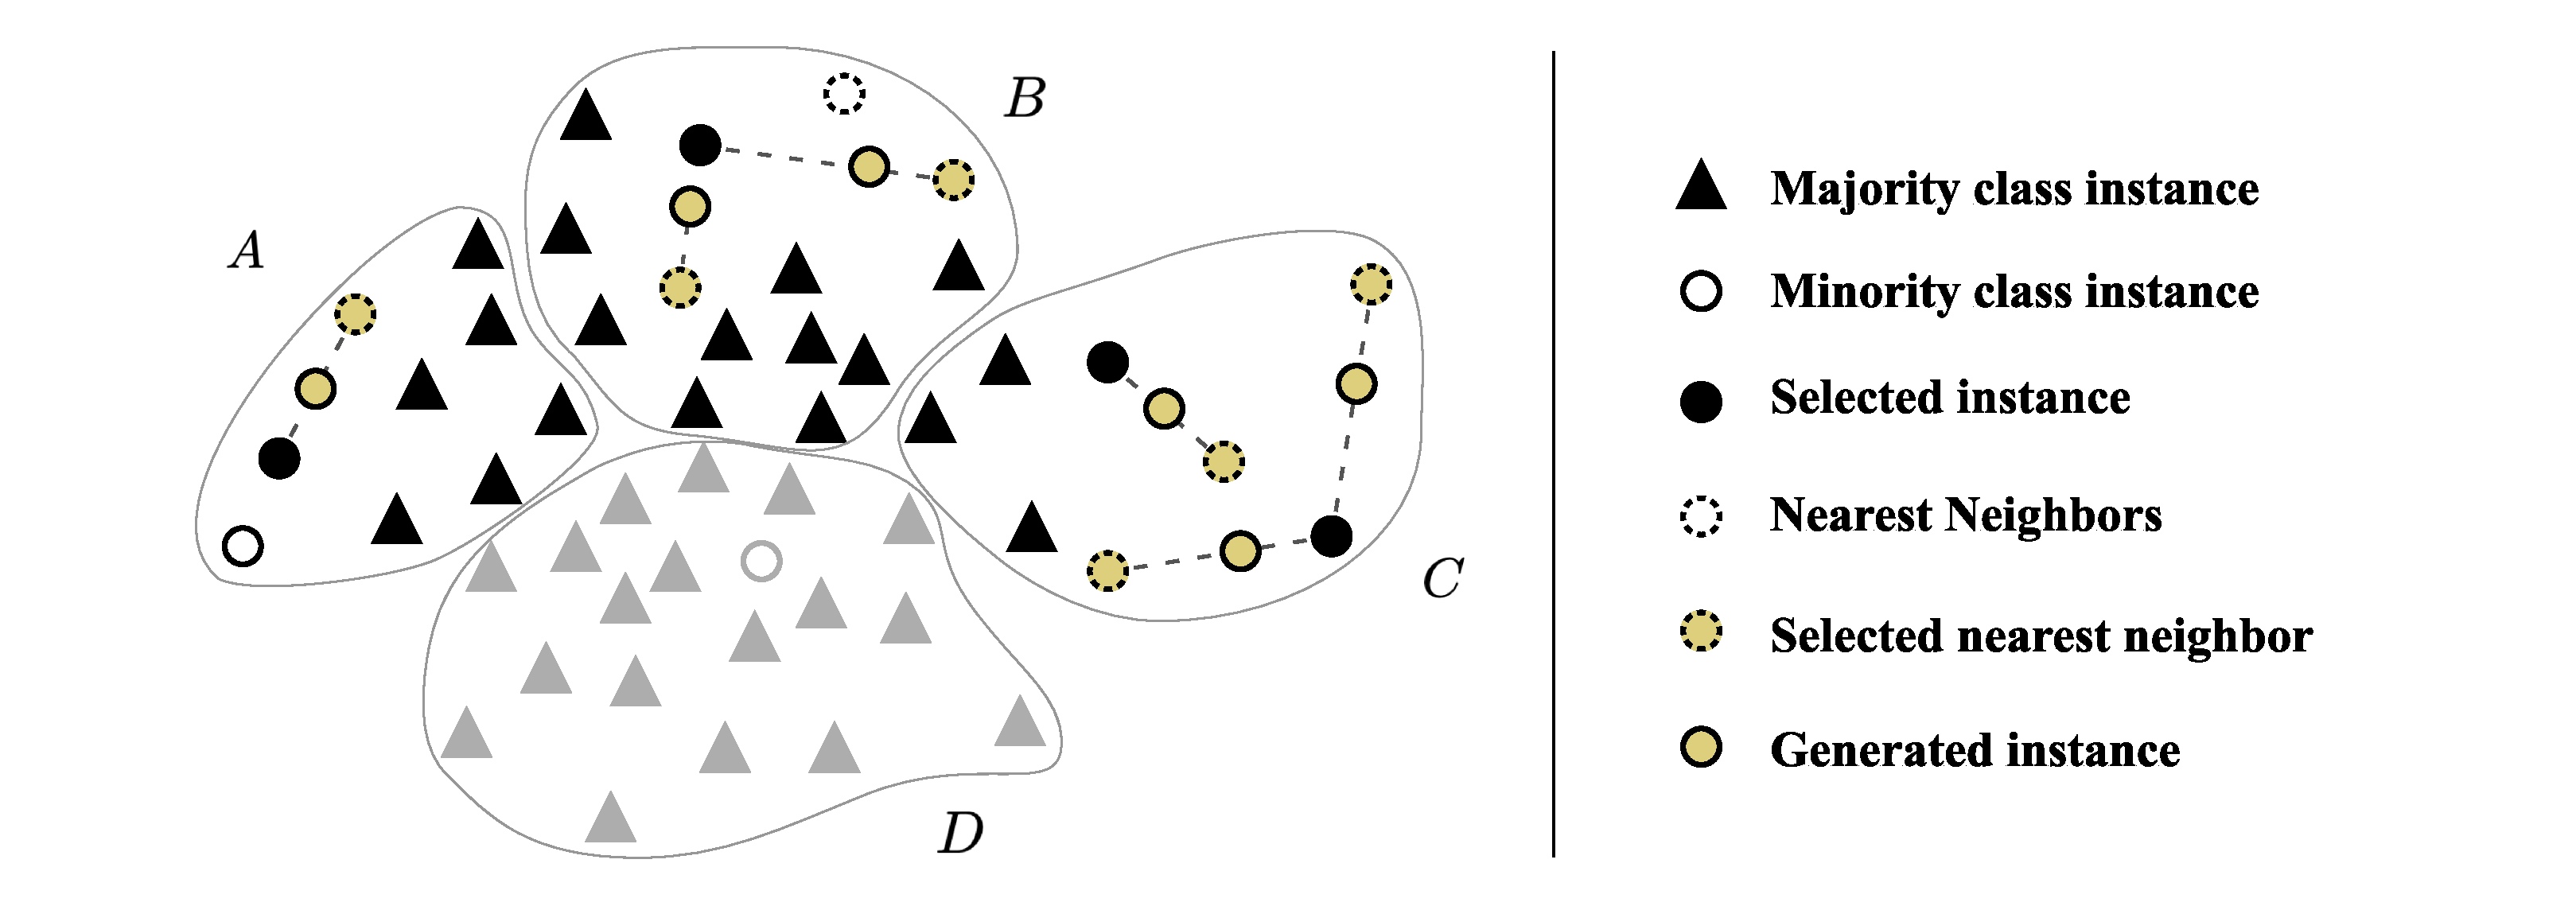
\includegraphics[width=1\linewidth]{../analysis/kmeans_smote_example}
\end{figure}
\begin{paracol}{2}
\linenumbers
\switchcolumn

K-means SMOTE~\citep{Douzas2018} avoids noisy data generation by modifying the
data selection mechanism. It employs $k$-means clustering to identify safe
areas using cluster-specific Imbalance Ratio (IR, defined by
$\frac{count(C_{majority})}{count(C_{minority})}$) and determine the quantity
of generated samples per cluster based on a density measure. These samples are
finally generated using the SMOTE algorithm. The K-means SMOTE's data
generation process is depicted in Figure~\ref{fig:kmeans_smote_example}. Note
that the number of samples generated for each cluster varies according to the
sparsity of each cluster (the sparser the cluster is, the more samples will be
generated) and a cluster is rejected if the cluster's IR surpasses the
threshold.  Therefore, this method can be combined with any data generation
mechanism, such as G-SMOTE.  Also K-means SMOTE includes the SMOTE algorithm
as a special case when the number of clusters is set to one. Consequently,
K-means SMOTE returns results as good as or better than SMOTE.

Although no other study was found to implement cluster-based oversampling,
another study \citep{Douzas2019rs} compared the performance of SMOTE, ROS,
ADASYN, B-SMOTE and G-SMOTE in a highly imbalanced LULC classification dataset.
The authors found that G-SMOTE consistently outperformed the remaining
oversampling algorithms regardless of the classifier used.

\section{Methodology}\label{sec:methodology}

The purpose of this work is to understand the performance of K-means SMOTE as
opposed to other popular and/or state-of-the-art oversamplers for LULC
classification. This is done using 7 datasets with predominantly land use
information, along with 3 evaluation metrics and 3 classifiers to evaluate the
performance of oversamplers. In this section we describe the datasets,
evaluation metrics, oversamplers, classifiers and software used as well as the
procedure developed.

\subsection{Datasets}

The datasets used were extracted from publicly available hyperspectral scenes.
Information regarding each of these scenes is provided in this subsection.
The data collection and preprocessing pipeline is shown in
Figure~\ref{fig:data_preprocessing_pipeline} and is common to all
hyperspectral scenes:

\begin{enumerate}
    
    \item Data collection of publicly available hyperspectral scenes.
        The original hyperspectral scenes and ground truth data were collected
        from a single publicly available data repository available
        \href{http://www.ehu.eus/ccwintco/index.php?title=Hyperspectral_Remote_Sensing_Scenes}{here}.

    \item Conversion of each hyperspectral scene to a structured
        dataset and removal of instances with no associated LULC class. This
        done to reshape the dataset from $(h,w,b+gt)$  into a conventional
        dataframe of shape $(h*w,b+gt)$, where $gt$, $h$, $w$ and $b$
        represents the ground truth, height, width and number of bands in the
        scene, respectively. The pixels without ground truth information are
        discarded from further analysis.

    \item Stratified random sampling to maintain similar class
        proportions on a sample of 10\% of each dataset. This is done by
        computing the relative class frequencies in the original hyperspectral
        scene (minus the class representing no ground truth availability) and
        retrieving a sample that ensures the original relative class
        frequencies remain unchanged.

    \item Removal of instances belonging to a class with frequency
        lower than 20 or higher than 1000. This is done to maintain the
        datasets to a practicable size due to computational constraints, while
        conserving the relative LULC class frequencies and data distribution. 

    \item Data normalization using the MinMax scaler. This ensures all
        features (i.e., bands) are in the same scale. In this case, the data
        was rescaled between 0 and 1.

\end{enumerate}

Table~\ref{tab:datasets_description} provides a description of the final
datasets used for this work, sorted according to its IR.
Figure~\ref{fig:scenes} shows the original hyperspectral scene out of which
the dataset used in this experiment were extracted. In the representation of
the ground truth of these scenes, the blue regions in the ground truth of each
hyperspectral scene represent unlabeled regions (i.e., no  ground truth is
available). Particularly, in the Botswana and Kennedy Space Center scenes the
truth was photointerpreted in more limited regions of the scene. However, the
scenes are still represented as they are in order to maintain a standardized
analysis over all datasets extracted for the experiment.

\end{paracol}
\begin{figure}
	\centering
    \captionsetup{justification=centering}
    \caption{Data collection and preprocessing pipeline.
    \vspace{.2cm}}
	\label{fig:data_preprocessing_pipeline}
	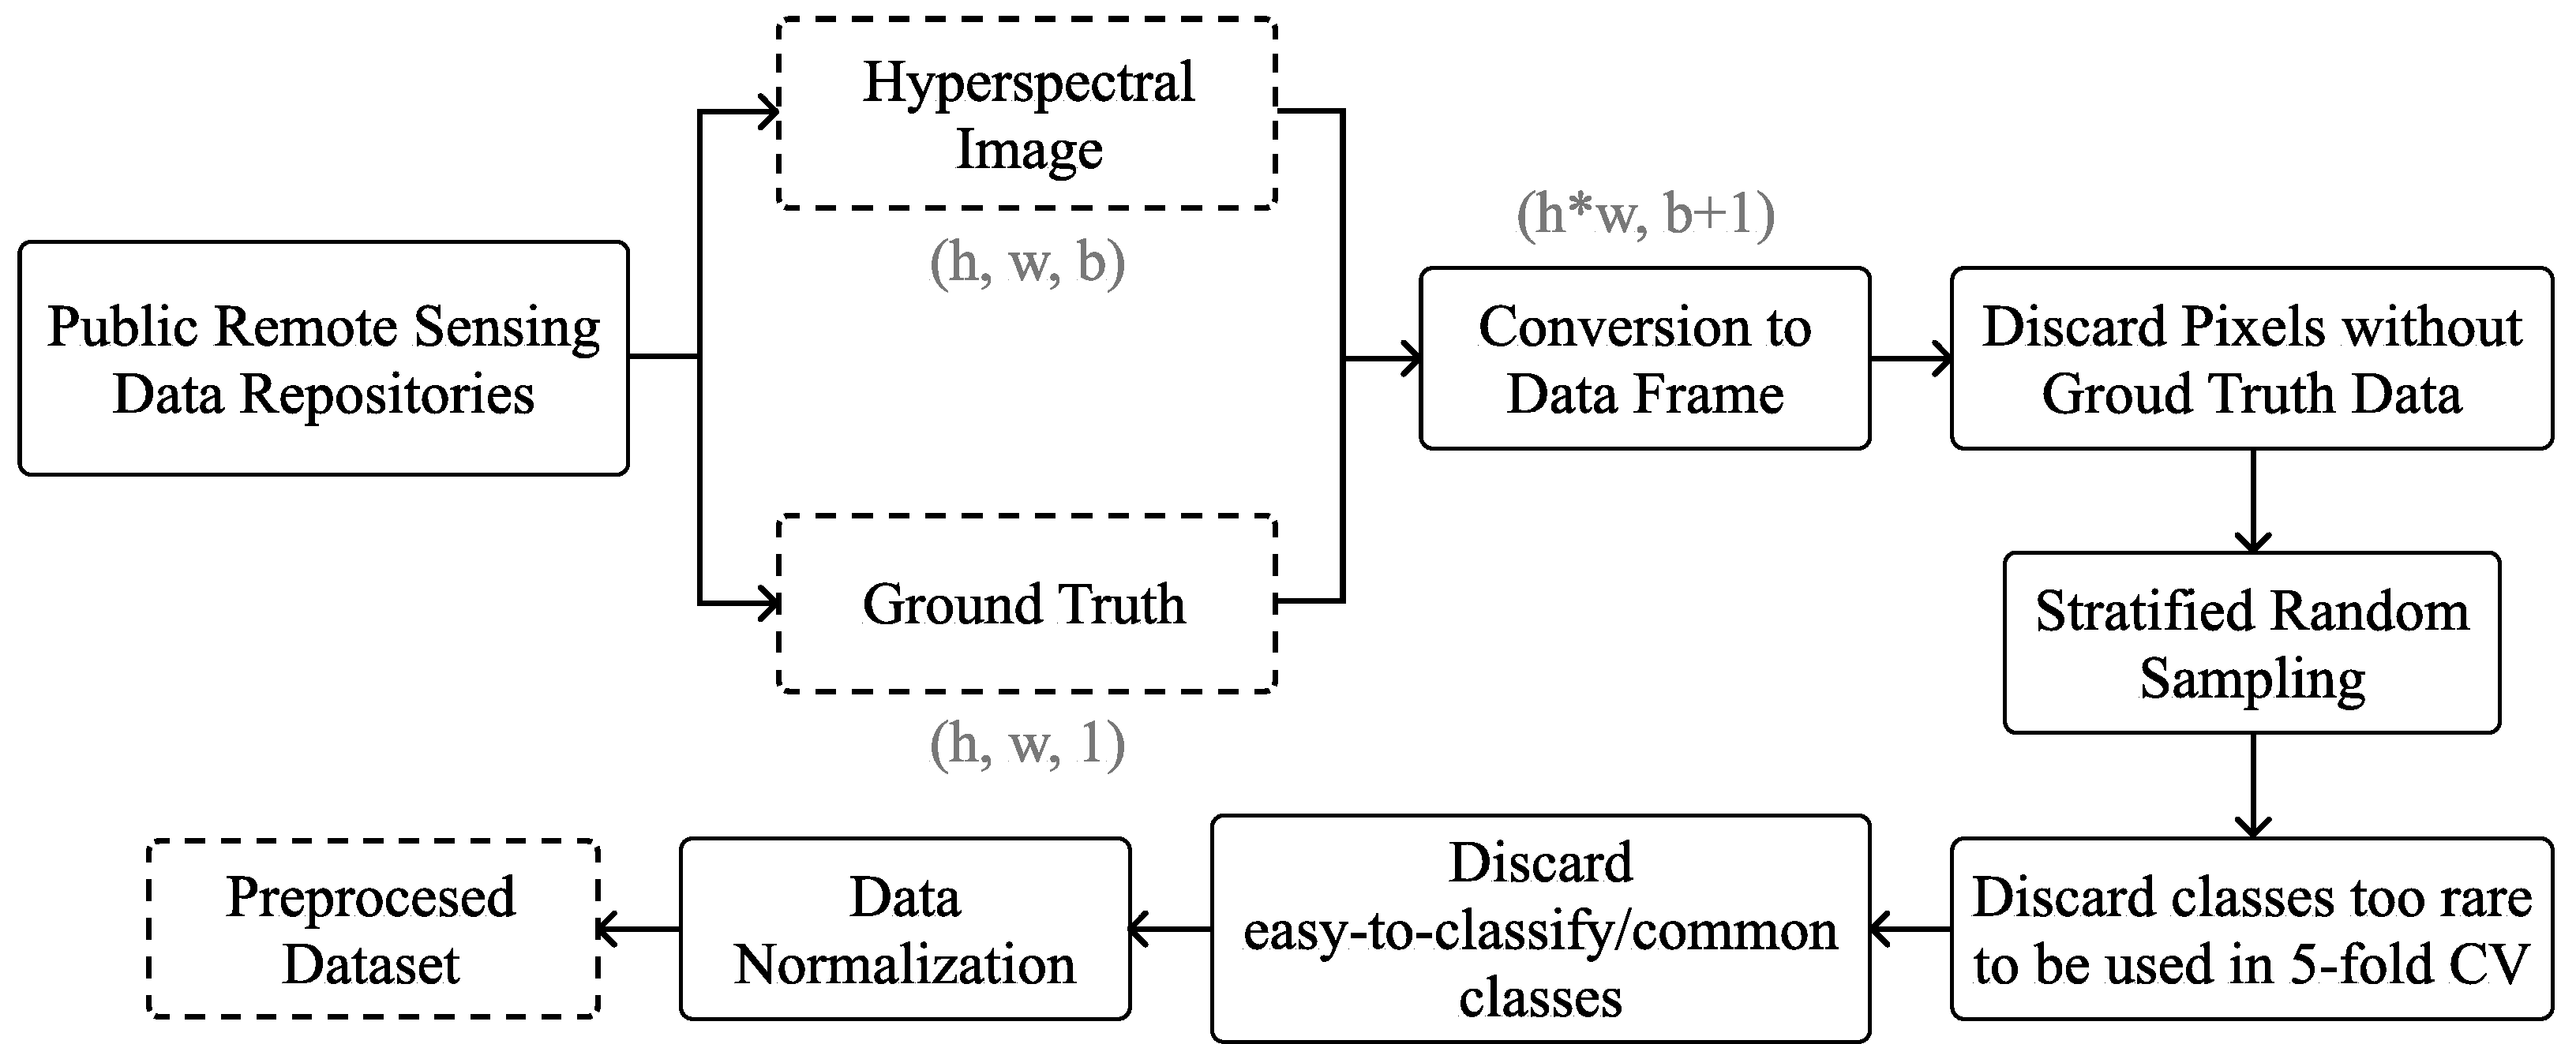
\includegraphics[width=.75\linewidth]{../analysis/data_preprocessing_pipeline}
\end{figure}
\begin{paracol}{2}
\linenumbers
\switchcolumn

\end{paracol}
\begin{table}
	\centering
    \addtolength{\leftskip} {-2cm}
    \addtolength{\rightskip}{-2cm}
    \captionsetup{justification=centering}
    \caption{Description of the datasets used for this
    experiment.\label{tab:datasets_description}}
    \pgfplotstabletypeset[
        col sep=comma,
        string type,
        every head row/.style={%
            before row=\toprule,
            after row=\midrule
        },
        every last row/.style={after row=\bottomrule},
        string type,
    ]{../analysis/datasets_description.csv}
\end{table}
\begin{paracol}{2}
\linenumbers
\switchcolumn

\subsubsection*{Botswana}

The Botswana scene was acquired by the Hyperion sensor on the NASA EO-1
satellite over the Okavango Delta, Botswana in 2001-2004 at a 30m spatial
resolution. Data preprocessing was performed by the UT Center for Space
Research. The scene comprises a $1476 \times 256$ pixels with 145 bands and 14
classes regarding land cover types in seasonal and occasional swamps, as well
as drier woodlands (see Figure~\ref{fig:botswana}). The classes with
rare instances are Short mopane and Hippo grass.

\subsubsection*{Pavia Center and University}

Both Pavia Center and University scenes were acquired by the ROSIS sensor.
These scenes are located in Pavia, northern Italy. Pavia Center is a $1096
\times 1096$ pixels image with 102 spectral bands, whereas Pavia University is
a $610 \times 610$ pixels image with 103 spectral bands. Both images have a
geometrical resolution of 1.3m and their ground truths are
composed of 9 classes each (see Figures~\ref{fig:pavia_center}
and~\ref{fig:pavia_university}). After data preprocessing, the classes
with rare instances are Asphalt and Bitumen (the class Shadows was removed for
being too rare for cross validation after random sampling).

\subsubsection*{Kennedy Space Center}

The Kennedy Space Center scene was acquired by the AVIRIS sensor over the
Kennedy Space Center, Florida, on March 23, 1996. Out of the original 224
bands, water absorption and low SNR bands were removed and a total of 176
bands at a spatial resolution of 18m are used. The scene is a $512 \times 614$
pixel image and contains a total of 16 classes (see
figure~\ref{fig:kennedy_space_center}). The classes with rare instances
are hardwood swamp, slash pine and willow swamp (both hardwood swamp and slash
pine were removed for being too rare for cross validation after random
sampling).

\subsubsection*{Salinas and Salinas-A}

These scenes were collected by the AVIRIS sensor over Salinas Valley,
California and contain at-sensor radiance data. Salinas is a $512 \times 217$
pixels image with 224 bands and 16 classes regarding vegetables, bare soil and
vineyard fields (see Figure~\ref{fig:salinas}). Salinas-A, a subscene of
Salinas, comprises $86 \times 83$ pixels and contains 6 classes regarding
vegetables (see Figure~\ref{fig:salinas_a}). These scenes have a geometrical
resolution of 3.7m. Salinas-A's minority class has the label
``Brocoli\_green\_weeds\_1'' and Salina's minority class has the label
``Lettuce\_romaine\_6wk''

\subsubsection*{Indian Pines} 

The Indian Pines scene~\citep{Baumgardner2015} was collected on June 12, 1992
and consists of AVIRIS hyperspectral image data covering the Indian Pine Test
Site 3, located in North-western Indiana, USA. As a subset of a larger scene,
it is composed of $145 \times 145$ pixels (see Figure~\ref{fig:indian_pines})
and 220 spectral reflectance bands in the wavelength range 400 to 2500
nanometers at a spatial resolution of 20m. Approximately two thirds of
this scene is composed by agriculture and the other third is composed of
forest and other natural perennial vegetation. Additionally, the scene also
contains low density buildup areas. The classes with rare instances are
Alfalfa, Oats, Grass-pasture-mowed, Wheat and Stone-Steel-Towers (which
removed for being too rare for cross validation after random sampling).  After
data preprocessing, the classes with rare instances are Corn,
Buildings-Grass-Trees-Drives and Grass-Pasture.

\pagebreak
\end{paracol}
\begin{figure}[H]
	\centering
    \captionsetup{justification=centering}
    \caption{Gray scale visualization of a band (top row) and ground truth
        (bottom row) of each scene used in this study. (a) Botswana, (b) Pavia
        Center, (c) Pavia University, (d) Kennedy Space Center,
        (e) Salinas, (f) Salinas A, (g) Indian Pines.
    \vspace{.25cm}}\label{fig:scenes}
	
	\begin{subfigure}{.24\textwidth}
		\centering
		\captionsetup{skip=12pt,justification=centering}
		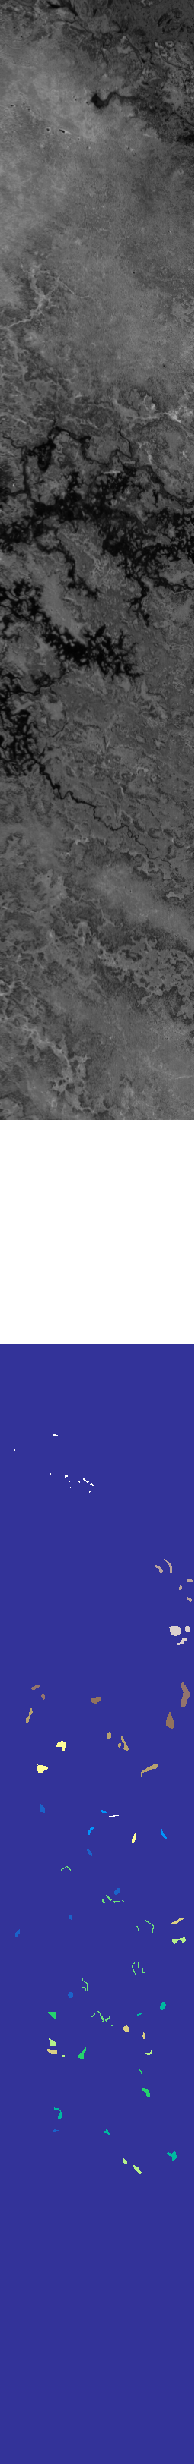
\includegraphics[height=1.5\linewidth]{../analysis/botswana}
		\subcaption{{\medbreak}}\label{fig:botswana}
	\end{subfigure}
	\begin{subfigure}{.24\textwidth}
		\centering
		\captionsetup{skip=12pt,justification=centering}
		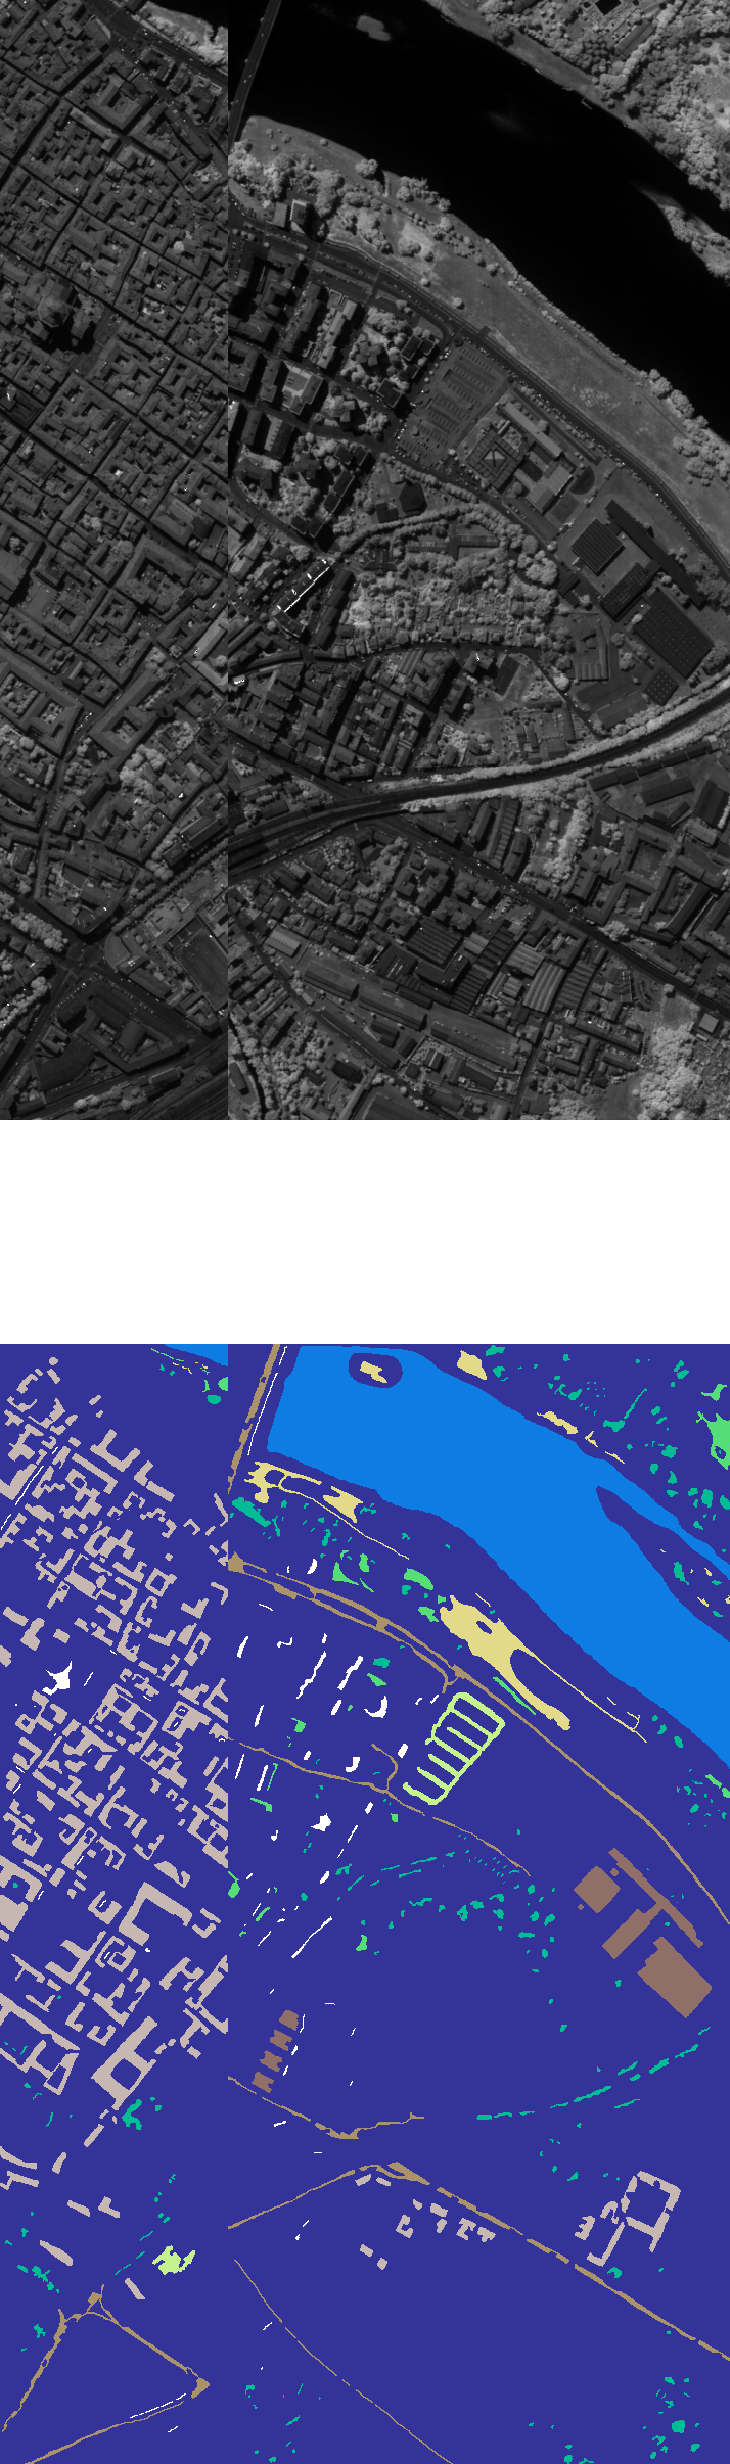
\includegraphics[height=1.5\linewidth]{../analysis/pavia_centre}
		\subcaption{{\medbreak}}\label{fig:pavia_center}
	\end{subfigure}
	\begin{subfigure}{.24\textwidth}
		\centering
		\captionsetup{skip=12pt,justification=centering}
		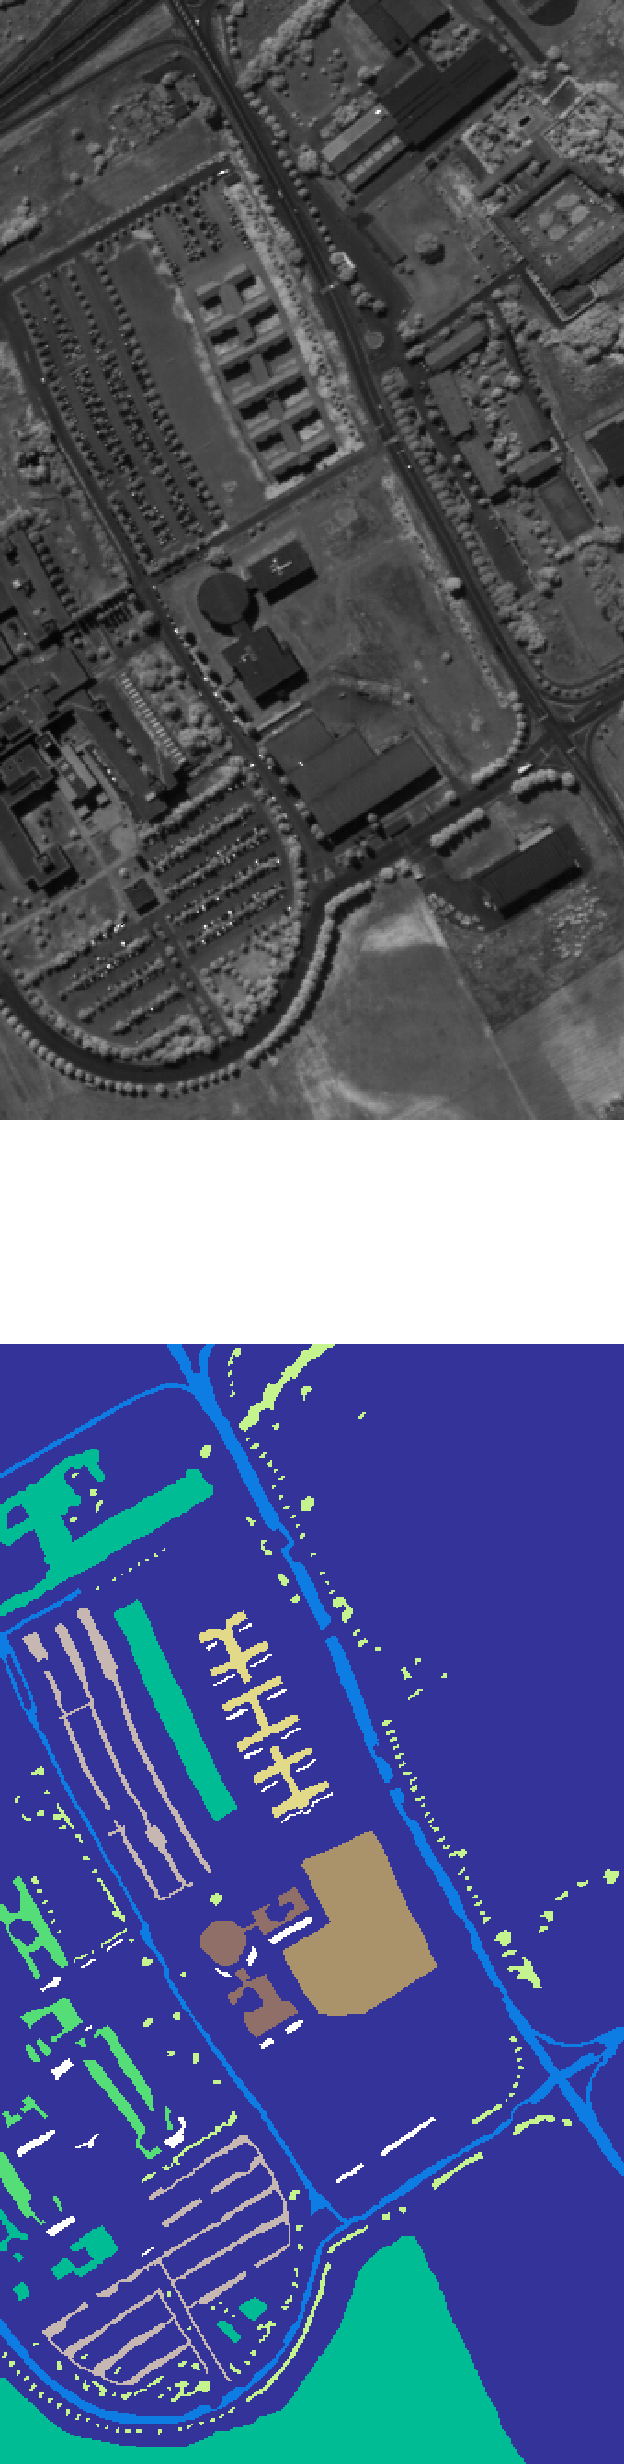
\includegraphics[height=1.5\linewidth]{../analysis/pavia_university}
		\subcaption{{\medbreak}}\label{fig:pavia_university}
	\end{subfigure}
	\begin{subfigure}{.24\textwidth}
		\centering
		\captionsetup{skip=12pt,justification=centering}
		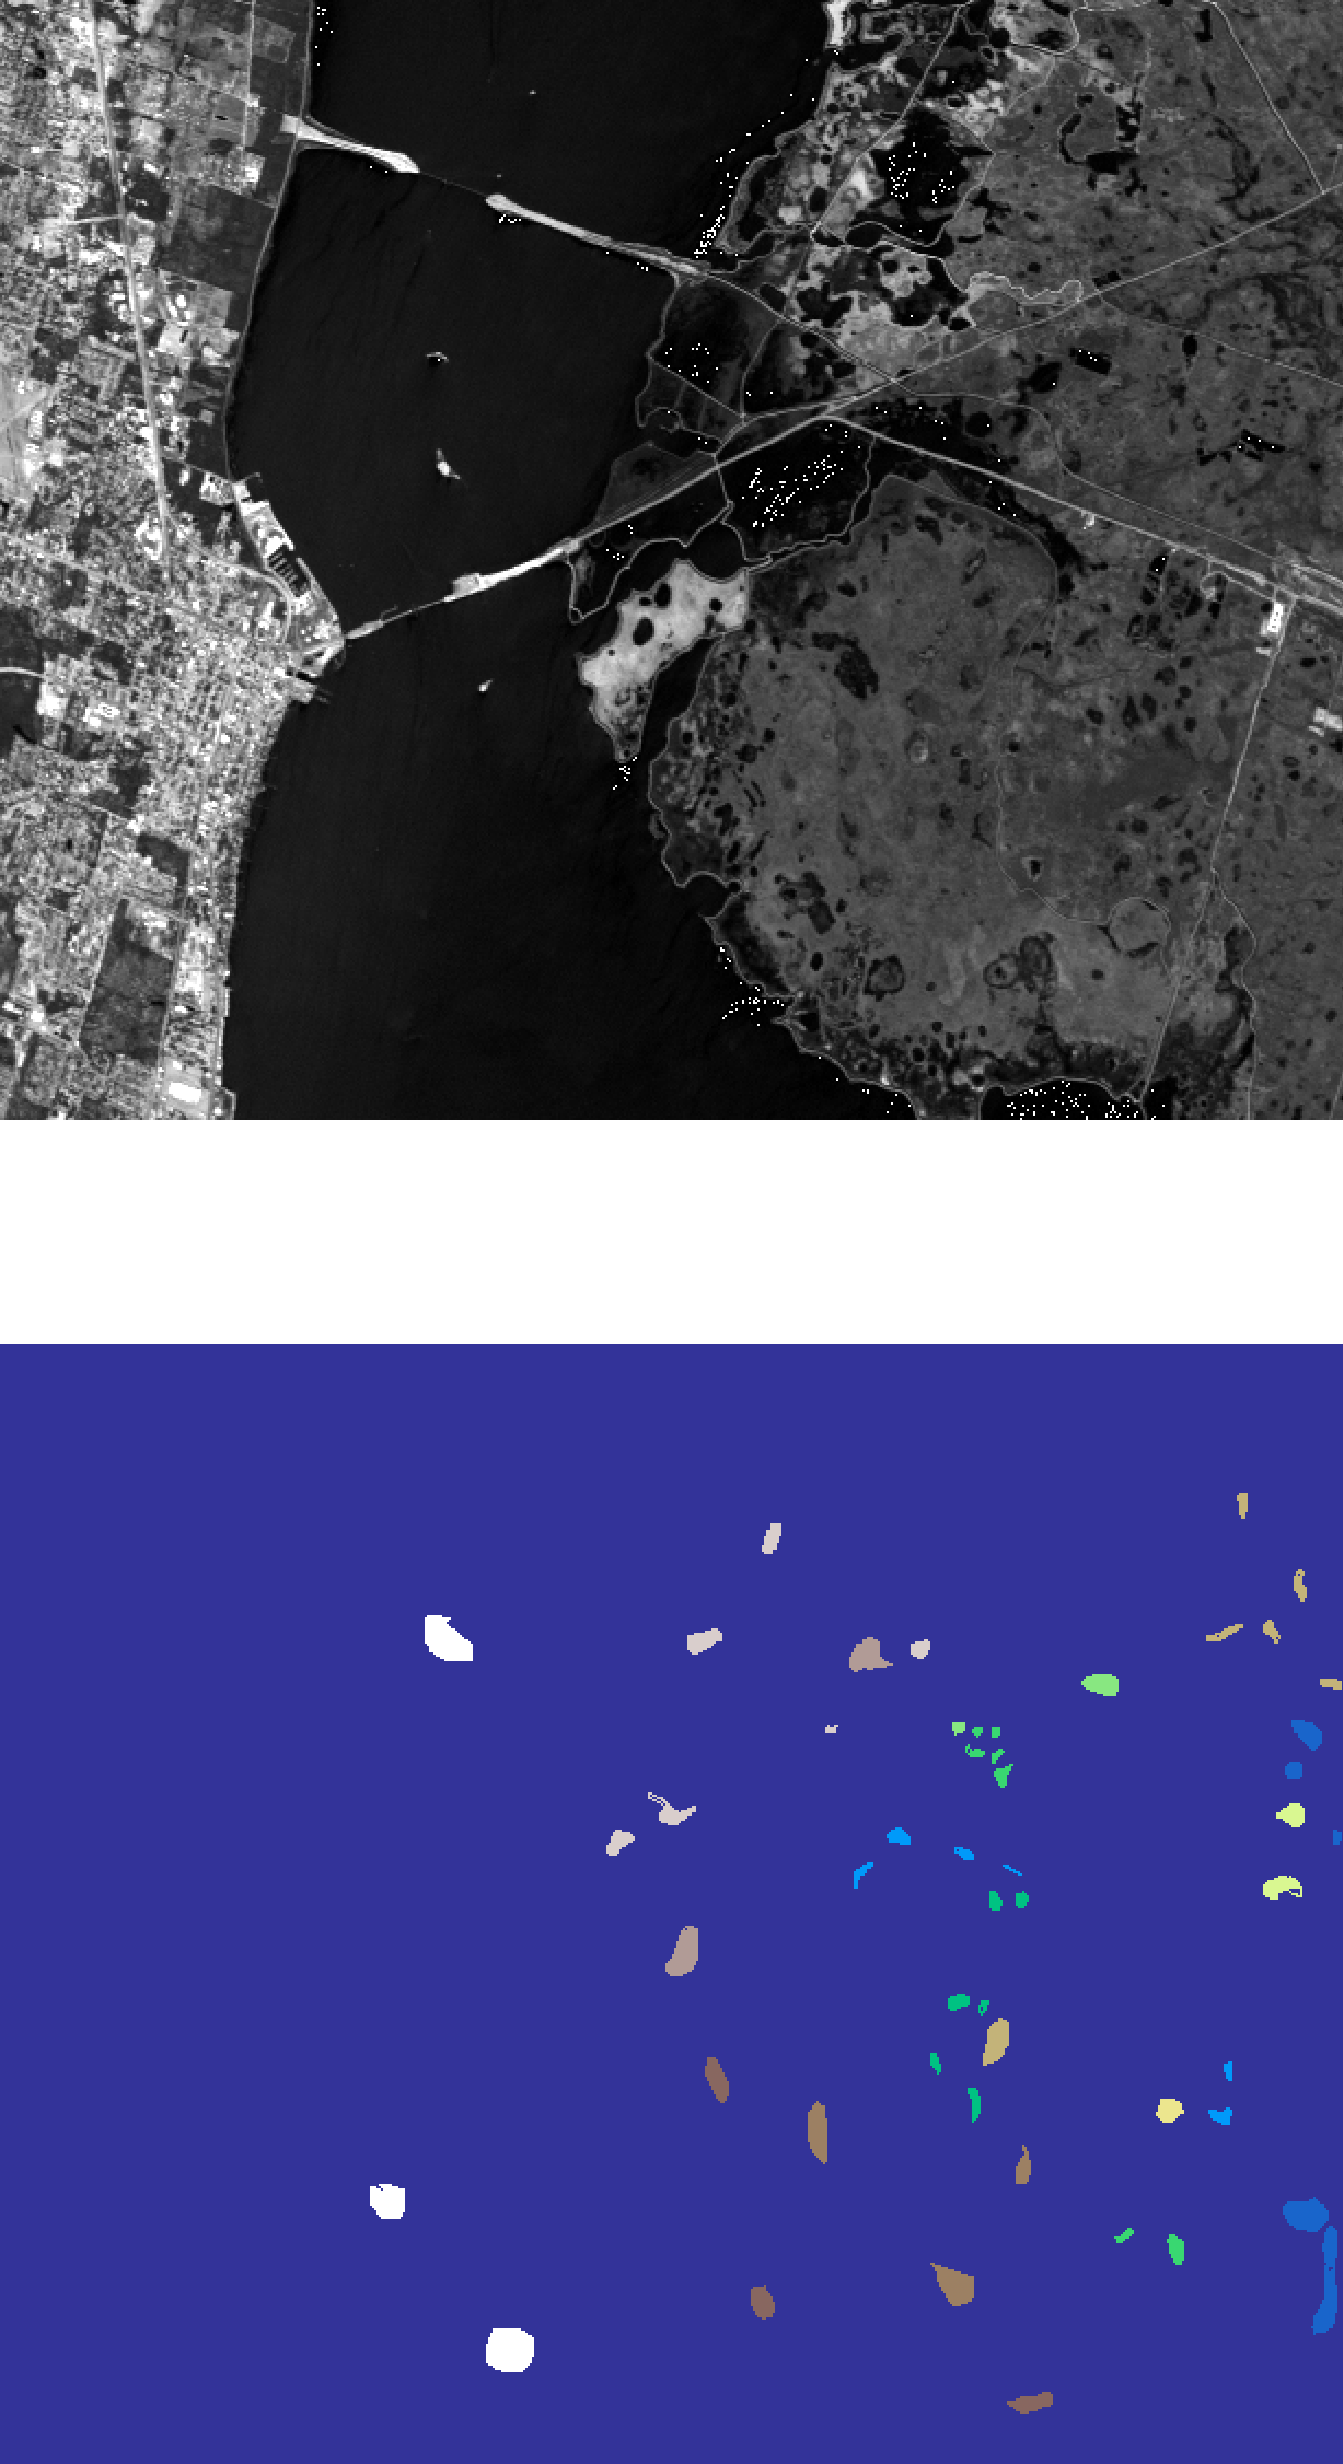
\includegraphics[height=1.5\linewidth]{../analysis/kennedy_space_center}
		\subcaption{{\medbreak}}\label{fig:kennedy_space_center}
	\end{subfigure}

	\begin{subfigure}{.24\textwidth}
		\centering
		\captionsetup{skip=12pt,justification=centering}
		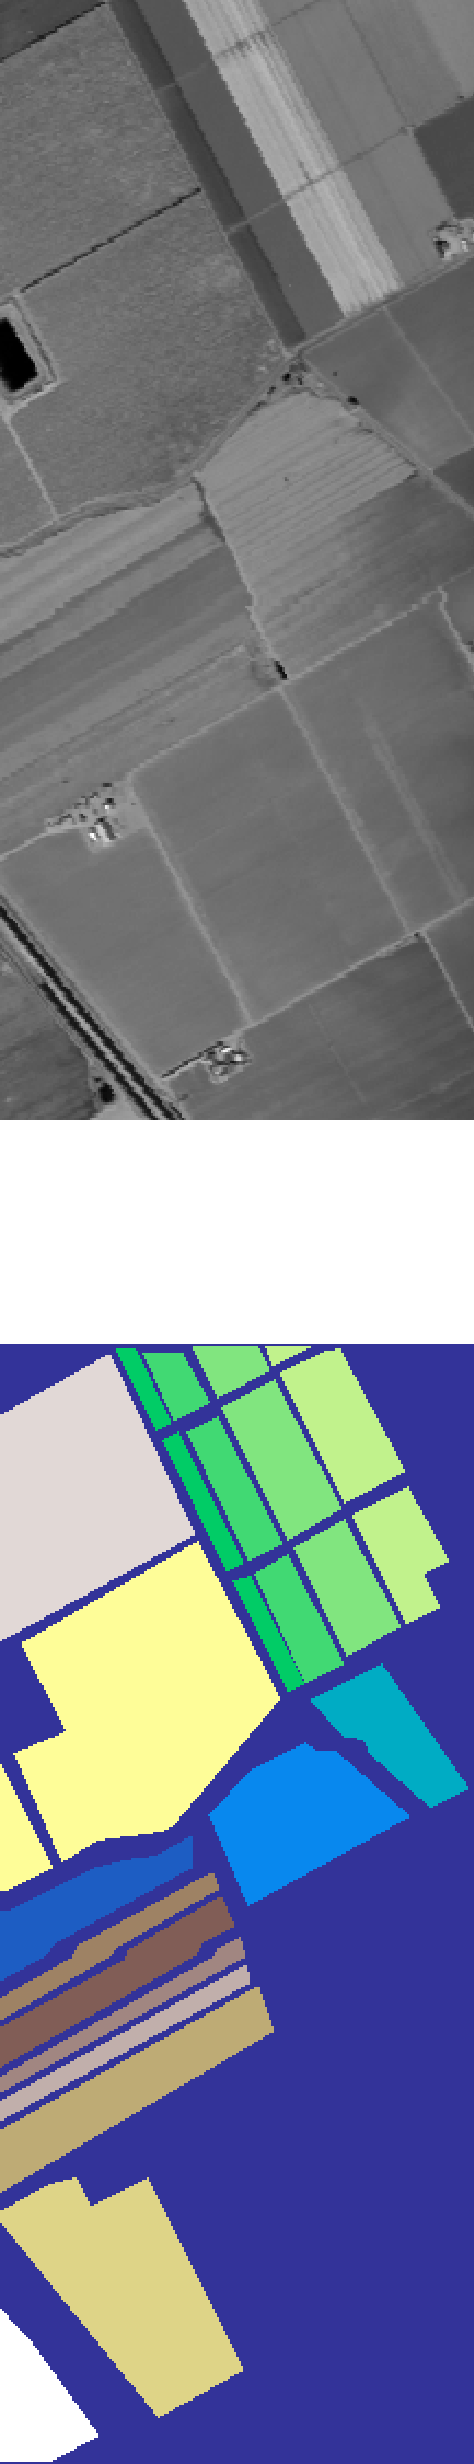
\includegraphics[height=1.5\linewidth]{../analysis/salinas}
		\subcaption{{\medbreak}}\label{fig:salinas}
	\end{subfigure}
	\begin{subfigure}{.24\textwidth}
		\centering
		\captionsetup{skip=12pt,justification=centering}
		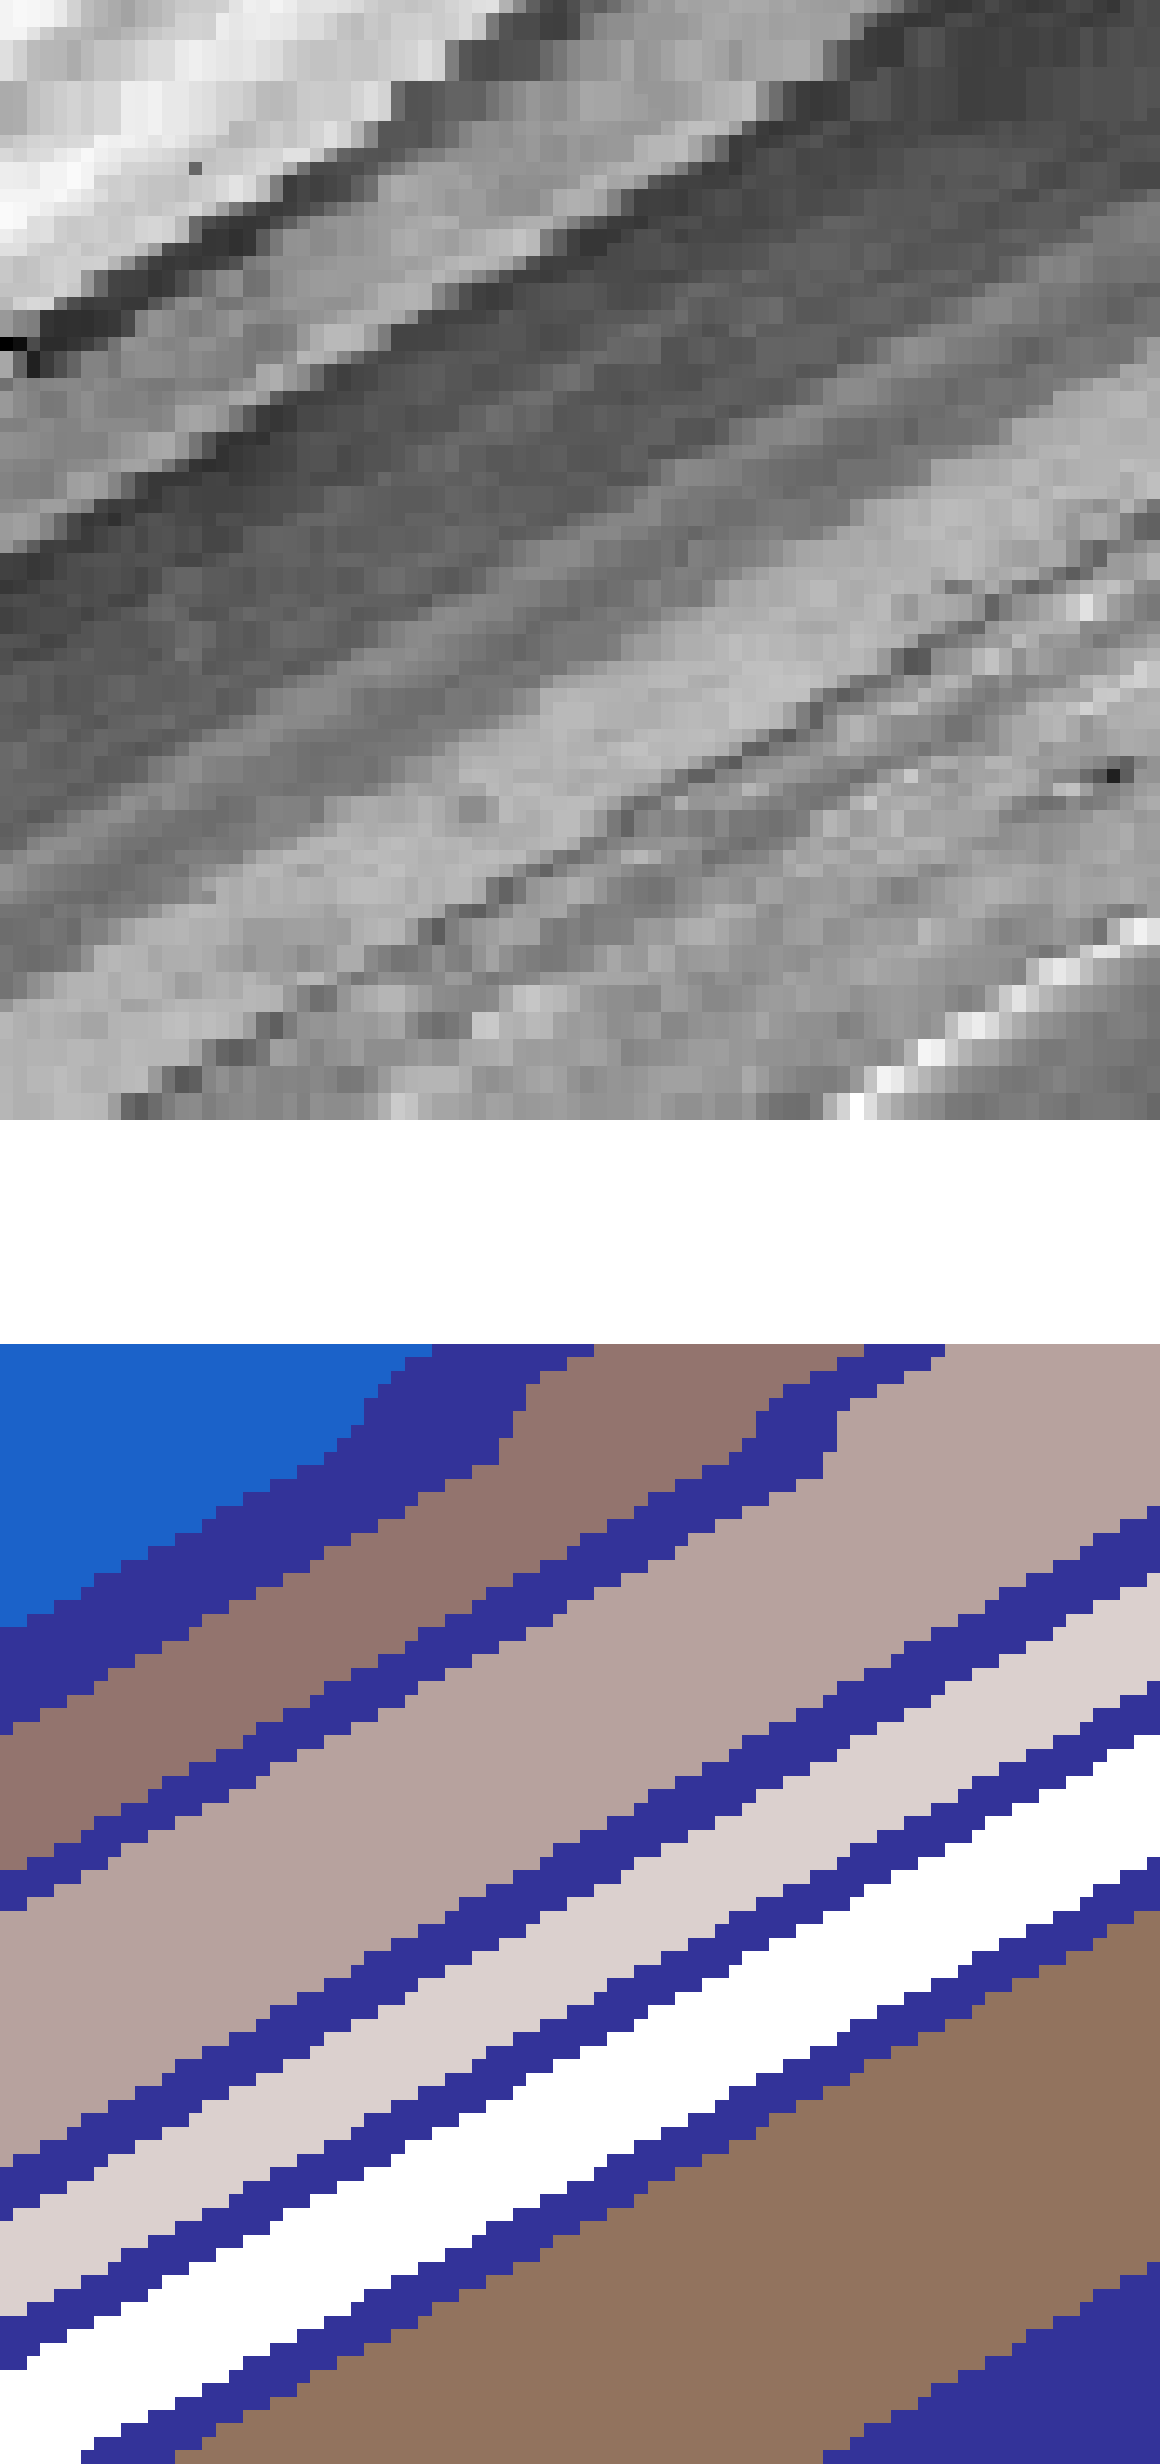
\includegraphics[height=1.5\linewidth]{../analysis/salinas_a}
		\subcaption{{\medbreak}}\label{fig:salinas_a}
	\end{subfigure}
    \begin{subfigure}{.24\textwidth}
		\centering
		\captionsetup{skip=12pt,justification=centering}
		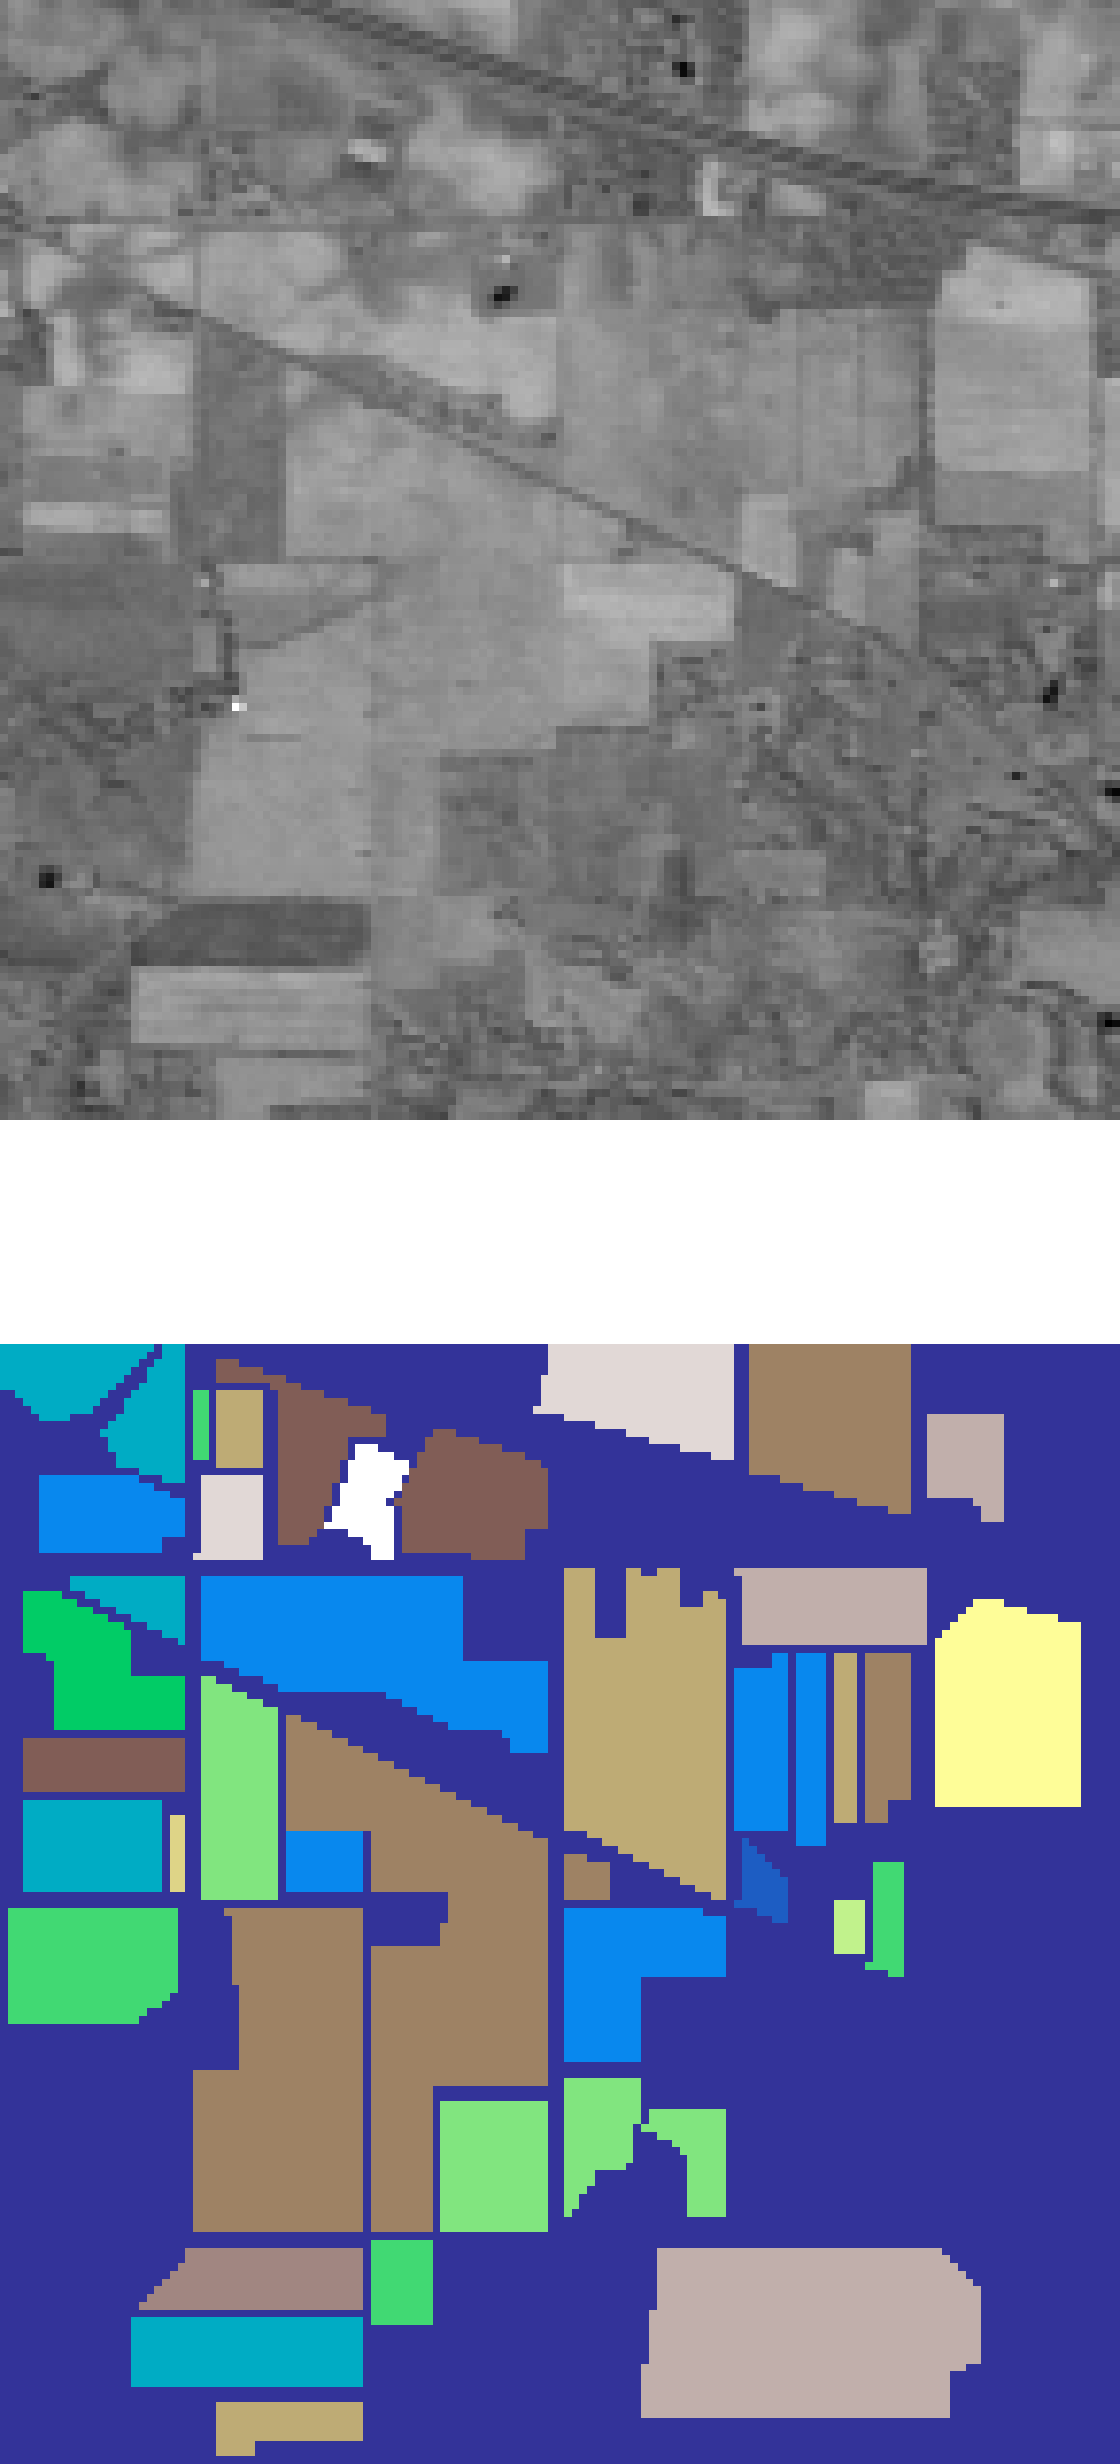
\includegraphics[height=1.5\linewidth]{../analysis/indian_pines}
		\subcaption{{\medbreak}}\label{fig:indian_pines}
	\end{subfigure}
\end{figure}
\begin{paracol}{2}
\linenumbers
\switchcolumn

\subsection{Machine Learning Algorithms}

To assess the quality of the K-means SMOTE algorithm,
three other oversampling algorithms were used for benchmarking. ROS and SMOTE
were chosen for their simplicity and popularity. B-SMOTE chosen as a popular
variation of the SMOTE algorithm. We also include the classification results
of no oversampling (NONE) as a baseline.

To assess the performance of each oversampler, we use the classifiers Logistic
Regression (LR) \citep{Nelder1972}, K-Nearest Neighbors (KNN)
\citep{Cover1967} and Random Forest (RF)
\citep{Liaw2002}. This choice was based on the classifiers' popularity for LULC
classification, learning type and training time
\citep{Maxwell2018,Gavade2019}. Since this is a multinomial classification
task, for the LR classification we adopted a one-versus-all approach for each
label. The predicted label is assigned according to the class predicted with
highest probability.

\subsection{Evaluation Metrics}~\label{sec:evaluation-metrics}

Most of the satellite-based LULC classification studies (nearly 80\%) employ
\textit{Overall Accuracy} (OA) and the \textit{Kappa Coefficient}
\citep{Gavade2019}. Although, some authors argue that both evaluation metrics,
even when used simultaneously, are insufficient to fully address the area
estimation and uncertainty information needs \citep{Olofsson2013,Pontius2011}.
Other metrics like User's Accuracy (or \textit{Precision}) and Producer's
Accuracy (or \textit{Recall}) are also common metrics to evaluate per-class
prediction power. These metrics consist of ratios employing the True and False
Positives (\textit{TP} and \textit{FP}, number of correctly/incorrectly
classified instances of a given class) and True and
False Negatives (\textit{TN} and \textit{FN}, number of correctly/incorrectly
classified instances as not belonging to a given
class). These metrics are formulated as $Precision = \frac{TP}{TP+FP}$ and
$Recall = \frac{TP}{TP+FN}$. While metrics like OA and \textit{Kappa
Coefficient} are significantly affected by imbalanced class distributions,
\textit{F-Score} is less sensitive to data imbalance and a more appropriate
choice for performance evaluation \citep{Jeni2013}.

The datasets used present significantly high IRs (see Table
\ref{tab:datasets_description}). Therefore, it is especially important to
attribute equal importance to the predictive power of all classes, which does
not happen with OA and \textit{Kappa Coefficient}. In this study, we employ 3
evaluation metrics: 1) \textit{G-mean}, since it is not affected by skewed class
distributions, 2) \textit{F-Score}, as it proved to be a more appropriate metric
for this problem when compared to other commonly used metrics \citep{Jeni2013},
and 3) \textit{Overall Accuracy}, for discussion purposes.

\begin{itemize}
    \item The \textit{G-mean} consists of the geometric mean of $Specificity =
        \frac{TN}{TN + FP}$ and \textit{Sensitivity} (also known as
        \textit{Recall}). For multiclass problems, The \textit{G-mean} is
        expressed as:

        $$\textit{G-mean} = \sqrt{ \overline{Sensitivity} \times
        \overline{Specificity}}$$

    \item \textit{F-score} is the harmonic mean of \textit{Precision} and
        \textit{Recall}. The \textit{F-score} for the multi-class case can be
        calculated using their average per class values \citep{He2009}:

          $$\textit{F-score}=2\frac{\overline{Precision} \times
          \overline{Recall}}{\overline{Precision} + \overline{Recall}}$$

    \item \textit{Overall Accuracy} is the number of correctly classified
        instances divided by the total amount of instances. Having \( c \) as
        the label of the various classes, \textit{Accuracy} is given by the
        following formula:

	      $$\textit{Accuracy} = \frac{ \sum\limits_{c}{ \text{TP}_{c} } }{
			      \sum\limits_{c}{ (\text{TP}_{c}  + \text{FP}_{c}) } } $$

\end{itemize}

In the case of \textit{G-mean} and \textit{F-score}, both metrics are computed
for each label and their unweighted mean is calculated (\textit{i.e.},
following a ``macro'' approach). In this study we assume that all labels
have an equivalent importance for the classification task.

\subsection{Experimental Procedure}

The procedure for the experiment started with the definition of a
hyperparameter search grid, where a list of possible values for each relevant
hyperparameter in both classifiers and oversamplers is stored. Based on this
search grid, all possible combinations of oversamplers, classifiers and
hyperparameters are formed.  Finally, for each dataset, hyperparameter
combination and initialization we use the evaluation strategy shown in Figure
\ref{fig:experiment_pipeline}: $k$-fold cross-validation strategy where $k=5$
to train each model defined and save the averaged scores of each split.

In the 5-fold cross validation strategy, a combination
of oversampler, classifier and hyperparameters vector is fit 5 times
per dataset. Before the training
phase, the training set
(containing $\frac{4}{5}$ of the dataset) is oversampled using one of the methods
described (except for the baseline method NONE), creating an augmented
dataset with the exact same number of instances for
each class. The newly formed training dataset is used to train the classifier
and the test set ($\frac{1}{5}$ of the dataset)
is used to evaluate the performance of the classifier. The evaluation scores
are then averaged over the 5 times the process is repeated. The range of
hyperparameters used are shown in table \ref{tab:grid}. The definition of
hyperparameters for the K-means SMOTE oversampler is defined according to the
recommendations discussed in the original K-means SMOTE
paper~\citep{Douzas2018}.

\end{paracol}
\begin{figure}
	\centering
    \captionsetup{justification=centering}
    \caption{Experimental procedure. The performance metrics are averaged over
    the 5 folds across each of the 3 different initializations of this
    procedure for a given combination of oversampler, classifier and
    hyperparameter definition.
    \vspace{.25cm}}\label{fig:experiment_pipeline}
	\includegraphics[width=1\linewidth]{../analysis/experiment_pipeline}
\end{figure}
\begin{paracol}{2}
\linenumbers
\switchcolumn

\end{paracol}
\begin{table}
	\centering
    \captionsetup{justification=centering}
    \caption{Hyper-parameters grid. $^*$~One cluster is generated in total, a
    corner case that mimics the behavior of SMOTE
    }\label{tab:grid}
    \begin{tabular}{lll}
		\toprule
		Classifier       & Hyperparameters      & Values                            \\
		\midrule
		LR               & maximum iterations   & 10000                             \\
		KNN              & \# neighbors  & {3, 5, 8}                            \\
		RF               & maximum depth        & {None, 3, 6}                      \\
		                 & \# estimators & {50, 100, 200}                         \\
		\toprule
		Oversampler      &                      &                                   \\
		\midrule
        K-means SMOTE    & \# neighbors  & {3, 5}                            \\
		                 & \# clusters (as \% of number of instances)   & {1$^*$, 0.1, 0.3, 0.5, 0.7, 0.9}      \\
                         & Exponent of mean distance & {auto, 2, 5, 7}       \\
                         & IR threshold  & {auto, 0.5, 0.75, 1.0}            \\
		SMOTE            & \# neighbors  & {3, 5}                            \\
		BORDERLINE SMOTE & \# neighbors  & {3, 5}                            \\
		\bottomrule
	\end{tabular}
\end{table}
\begin{paracol}{2}
\linenumbers
\switchcolumn

\subsection{Software Implementation}~\label{sec:implementation}

The experiment was implemented using the Python programming language, using the
\href{https://scikit-learn.org/stable/}{Scikit-Learn}~\citep{Pedregosa2011},
\href{https://imbalanced-learn.org/en/stable/}{Imbalanced-Learn}~\citep{JMLR:v18:16-365},
\href{https://geometric-smote.readthedocs.io/en/latest/?badge=latest}{Geometric-SMOTE},
\href{https://cluster-over-sampling.readthedocs.io/en/latest/?badge=latest}{Cluster-Over-Sampling}
and \href{https://research-learn.readthedocs.io/en/latest/?badge=latest}{Research-Learn} libraries.
All functions, algorithms, experiments and results are provided at the
\href{https://github.com/AlgoWit/publications}{GitHub
repository of the project}.

\section{Results \& Discussion}~\label{sec:results}

When evaluating the performance of an algorithm across multiple datasets, it
is generally recommended to avoid direct score comparisons and use
classification rankings instead~\citep{demvsar2006}. This is done by assigning
a ranking to oversamplers based on the different combinations of classifier,
metric and dataset used. These rankings are also used for the statistical
analyses presented in Section~\ref{sec:statistical_analysis}.

The rank values are assigned based on the mean validation scores resulting
from the experiment described in Section~\ref{sec:methodology}. The averaged
ranking results are computed over 3 different initialization seeds and a 5
fold cross validation scheme, returning a real number within the interval
$[1,5]$.

The hyperparameter optimization ensures that both oversamplers and classifiers
are well adapted to each of the datasets used in the experiment. Specifically,
the optimization of classifiers' hyperparameters is not particularly relevant
since our focus is to study the relative performance scores across
oversamplers. This will provide insights on the quality of the artificial data
generated by each oversampler. The classifiers' hyperparameter tuning was done
to avoid the over/underfitting of classifiers, since they are trained on the same
data subsets along with artificial data generated with different methods.

\subsection{Results}

The mean ranking of oversamplers is presented in
Figure~\ref{fig:mean_sem_ranking}. This ranking was computed by averaging the
ranks of the mean cross-validation scores per dataset, oversampler and
classifier. K-means SMOTE achieves the best mean ranking across datasets with
low standard deviation.


\end{paracol}
\begin{figure}[ht]
    \widefigure
    \captionsetup{justification=centering}
	\caption{
    	Results for mean ranking of oversamplers across datasets.
    \vspace{.2cm}}
	\label{fig:mean_sem_ranking}
	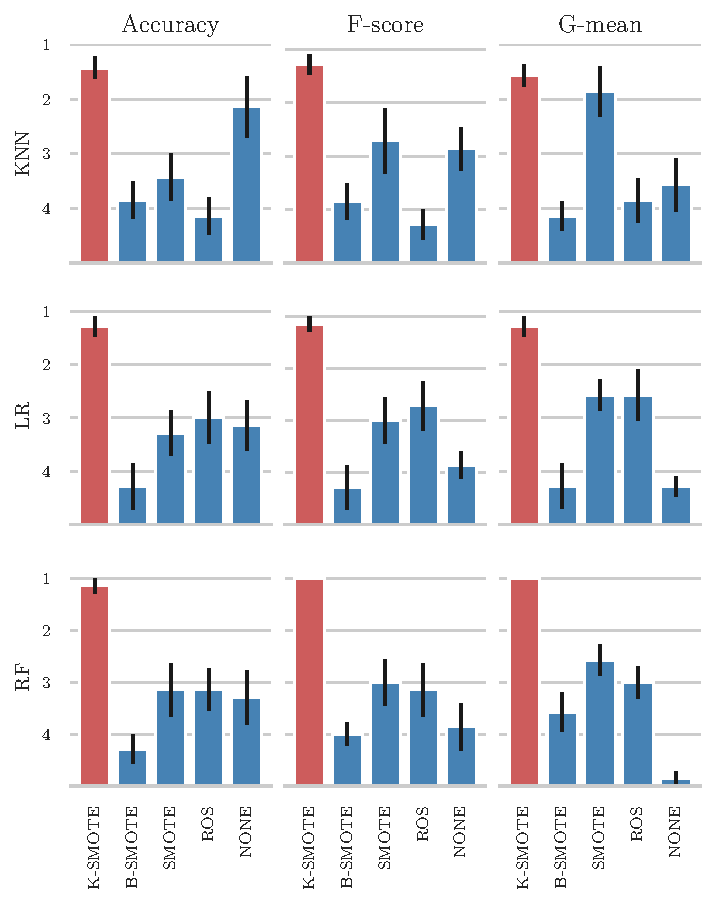
\includegraphics[width=.65\linewidth]{../analysis/mean_rankings_bar_chart}
\end{figure}
\begin{paracol}{2}
\linenumbers
\switchcolumn

The mean cross-validation scores are shown in Table~\ref{tab:mean_sem_scores}.
As discussed previously in this section, the disparity of performance levels
across datasets makes the analysis of these scores less informative.

\end{paracol}
\captionsetup{justification=centering}
\pgfplotstabletypeset[
	begin table=\begin{longtable},
	end table=\end{longtable},
	col sep=comma,
	header=true,
	columns={Classifier,Metric,NONE,ROS,SMOTE,B-SMOTE,K-SMOTE}, 
    string type,
    every head row/.style={before row={
    \caption{
		Mean cross-validation scores of oversamplers.
    }\label{tab:mean_sem_scores}\\
    \toprule}, after row=\midrule\endhead},
	every last row/.style={after row=\bottomrule}
]{../analysis/mean_sem_scores.csv}
\begin{paracol}{2}
\linenumbers
\switchcolumn

The mean cross-validation scores for each dataset are presented in
Table~\ref{tab:cross_validation_scores} (see appendix). This table allows the direct
comparison of the performance metrics being analysed.

\subsection{Statistical Analysis}~\label{sec:statistical_analysis}

The experiment's multi-dataset context was used to perform a Friedman
test~\citep{friedman1937use}. Table~\ref{tab:friedman_test} shows the results
obtained in the Friedman test performed, where the null hypothesis is rejected
in all cases. The rejection of the null hypothesis implies that the
differences between the differences among the different oversamplers are not
random, in other words, these differences are statistically significant.

\end{paracol}
\begin{table}[H]
    \caption{
        Results for Friedman test. Statistical significance is tested at a
        level of $\alpha = 0.05$. The null hypothesis is that there is no
        difference in the classification outcome across oversamplers.
    \vspace{-.6cm}}\label{tab:friedman_test}
    \pgfplotstabletypeset[
    	begin table=\begin{longtable},
    		end table=\end{longtable},  col sep=comma, header=true,
    	columns={Classifier,Metric,p-value,Significance}, string type, every head row/.style={before row=\toprule, after row=\midrule\endhead},
    	every last row/.style={after row=\bottomrule}
    ]{../analysis/friedman_test.csv}
\end{table}
\begin{paracol}{2}
\linenumbers
\switchcolumn

A Wilcoxon signed-rank test \citep{wilcoxon1992} was also performed to
understand whether K-means SMOTE's superiority was statistically significant
across datasets and oversamplers, as suggested in \citep{demvsar2006}. This
method is used as an alternative to the paired Student's t-test, since the
distribution of the differences between the two samples cannot be assumed as
normally distributed. The null hypothesis of the test is that K-means SMOTE's
performance is similar to the compared oversampler (i.e., the oversamplers
used follow a symmetric distribution around zero).

\pagebreak
\end{paracol}
\begin{table}[H]
    \caption{
        \textit{p-values} of the Wilcoxon signed-rank test. Boldface values
        are statistically significant at a significance level of $\alpha =
        0.05$.
    \vspace{-.6cm}}\label{tab:wilcoxon_test}
    \pgfplotstabletypeset[
    	begin table=\begin{longtable},
    		end table=\end{longtable},  col sep=comma, header=true,
    	columns={Dataset,NONE,ROS,SMOTE,B-SMOTE}, string type, every head row/.style={before row=\toprule, after row=\midrule\endhead},
    	every last row/.style={after row=\bottomrule}
    ]{../analysis/wilcoxon_test.csv}
\end{table}
\begin{paracol}{2}
\linenumbers
\switchcolumn

\subsection{Discussion}

The mean rankings presented in
Figure~\ref{fig:mean_sem_ranking} show that on average,
K-means SMOTE produced the best results for every classifier and performance
metric used. This is due to the clustering phase and subsequent selection of
data to be considered for oversampling. By successfully clustering and
selecting the relevant areas in the data space to oversample, the generation
of artificial instances is done only in the context of minority regions that
represent well their spectral signature.

As previously discussed, the direct comparison of performance metrics averaged
over various datasets is not recommended due to the varying levels of
performance of classifiers across datasets~\citep{demvsar2006}. Nonetheless,
these results are shown in Table~\ref{tab:mean_sem_scores} to provide a fuller
picture of the results obtained in the experiment. We found that on average
K-means SMOTE provides increased performance, regardless of the classifier and
performance metric used. More importantly, K-means SMOTE guaranteed a more
consistent performance across datasets and with less variability, which can be
attested in Figure~\ref{fig:mean_sem_ranking} and
Tables~\ref{tab:mean_sem_scores} and~\ref{tab:cross_validation_scores}.

As discussed in Subsection~\ref{sec:evaluation-metrics}, Evaluation Metrics,
our results are consistent with the findings in~\citep{Olofsson2013,
Pontius2011}. Particularly, we consider the results obtained in our experiment
using Overall Accuracy to be less informative than the results obtained with
the remaining performance metrics, since this metric is affected by imbalanced
class distributions. The majority class bias in this metric can be observed in
our experiment in Figure~\ref{fig:mean_sem_ranking} with the
classifiers LR and KNN, where the control method (NONE) is only outperformed
by K-means SMOTE. This effect is observed with more detail in
Table~\ref{tab:mean_sem_scores}, where the benchmark oversamplers are
outperformed by the control method in 16 out of 63 tests (approximately 25\%).
Out of these, most refer to tests using overall accuracy among the four
datasets with highest IR, showing the overall accuracy's class imbalance bias
discussed in~\citep{Olofsson2013, Pontius2011}. The K-means SMOTE oversampler
is only outperformed by the control method in 3 of tests (all of them using
overall accuracy). This is an improvement over the benchmark oversamplers,
showing that generally K-means SMOTE is the best choice even when overall
accuracy is used as the main performance metric.

In the majority of the cases, K-means SMOTE was able to generate higher
quality data due to the non-random selection of data spaces to oversample.
This can be seen in the performance of the classifiers trained on top of this
data generation step, making it a more informed data generation method in the
context of LULC\@.

The performance of both oversamplers and classifiers is generally dependent on
the dataset being used. Although both absolute and relative scores between the
different oversamplers are dependent on the choice of metric and classifier,
K-means SMOTE's relative performance is consistent across datasets and
generally outperforms the remaining oversampling methods in 56 of the 63 tests
(approximately 89\%). The mean cross-validation results found in
Table~\ref{tab:cross_validation_scores} show that performance-wise, K-means
SMOTE is always better than or as good as SMOTE, with the exception of 4
situations (representing 6\% of the tests done), in which cases the percentage
point difference is neglectable ($\leq 0.1$ percentage points). 

The statistical tests showed that not only there is a statistically
significant difference across the oversamplers used in this problem (found in
the Friedman test presented in Table~\ref{tab:friedman_test}), but also that
K-means SMOTE's superior performance is statistically significant at a level
of 0.05 in 27 out of 28 tests in the Wilcoxon signed-rank test shown in
Table~\ref{tab:wilcoxon_test} (approximately 96\% of the tests performed).
This shows that, in most cases, the usage of k-Means SMOTE improves the
quality of LULC classification when compared to using SMOTE in its original
format, which remains the most popular oversampler among the remote sensing
community.

Although the usage of K-means SMOTE successfully captured the spectral
signatures of the minority classes, it was done using K-means, a
problem-agnostic clusterer. Consequently, the implementation of this method
using a GIS-specific clusterer that considers the geographical traits of
different regions (e.g., using the sampled pixels' geographical coordinates),
may be a promising direction towards the development of more appropriate
oversampling techniques in the remote sensing domain.

\section{Conclusion}~\label{sec:conclusion} 

This research paper was motivated by the challenges faced when classifying
rare classes for LULC mapping. Cluster-based oversampling is especially useful
in this context because the spectral signature of a given class often varies,
depending on its geographical distribution and the time period within which
the image was acquired. This induces the representation of minority classes as
small clusters in the input space. As a result, training a classifier capable
of identifying LULC minority classes in the hyper/multi-spectral scene over
different areas or periods becomes particularly challenging. The clustering
procedure, performed before the data generation phase, allows for a more
accurate generation of minority samples, as it identifies these minority
clusters.

A number of existing methods to address the imbalanced learning problem were
identified and their limitations discussed. Typically, algorithm-based
approaches and cost-sensitive solutions are not only difficult to implement,
but they are also context dependent. In this paper we focused on oversampling
methods due to their widespread usage, easy implementation and flexibility.
Specifically, this paper demonstrated the efficacy of a recent oversampler,
K-Means SMOTE, applied in a multi-class context for Land Cover Classification
tasks. This was done with sampled data from seven well known and naturally
imbalanced benchmark datasets: Indian Pines, Pavia Center, Pavia University,
Salinas, Salinas A, Botswana and Kennedy Space Center. For each combination of
dataset, oversampler and classifier, the results of every classification task
was averaged across a 5 fold stratification strategy with 3 different
initialization seeds, resulting in a mean validation score of 15
classification tasks. The mean validation score of each combination was then
used to perform the analyses presented in this report.

In 56 out of 63 classification tasks (approximately 89\%), K-means SMOTE led
to better results than ROS, SMOTE, B-SMOTE and no oversampling. More
importantly, we found that K-Means SMOTE is always better or equal than the
second best oversampling method.  K-means SMOTE's performance was independent
from both the classifier and performance metric under analysis. In general,
K-means SMOTE shows a higher performance among the non tree-based classifiers
employed (LR and KNN) when compared with the remaining oversamplers, where
these oversamplers generally failed to improve the quality of classification.
Although these findings are case dependent, they are consistent with the
results presented in~\citep{Douzas2018}. The proposed method also had the most
consistent results across datasets, since it produced the lowest standard
deviations across datasets in 7 out of 9 cases for both analyses, either based
on ranking or mean cross-validation scores.

The proposed algorithm is a generalization of the original SMOTE algorithm. In
fact, the SMOTE algorithm represents a corner case of K-means SMOTE i.e., when
the number of clusters equals to 1. Its data selection phase differs from the
one used in SMOTE and Borderline SMOTE, providing artificially augmented
datasets with less noisy data than the commonly used methods. This allows the
training of classifiers with better defined decision boundaries, especially in
the most important regions of the data space (the ones populated by a higher
percentage of minority class instances).

As stated previously, the usage of this oversampler is technically simple. It
can be applied to any classification problem relying on an imbalanced dataset,
alongside any classifier. K-means SMOTE is available as an open source
implementation for the Python programming language (see
Subsection~\ref{sec:implementation}).  Consequently, it can be a useful tool
for both remote sensing researchers and practitioners.

\authorcontributions{Conceptualization, F.B.; Methodology, J.F. and G.D.; Software,
	J.F. and G.D.; Validation, F.B., G.D.; Formal Analysis, J.F; Writing -
	Original Draft Preparation, J.F.; Writing - Review \& Editing, F.B.,
	G.D., J.F.; Supervision, F.B.; Funding Acquisition, F.B.}

\funding{
    This research was funded by "Fundação para a Ciência e a Tecnologia"
    (Portugal), grants' number PCIF/SSI/0102/2017 - foRESTER and
    DSAIPA/AI/0100/2018 - IPSTERS.
}

\dataavailability{
    The data reported in this study is publicly available. It can be retrieved and
    preprocessed using the Python source code provided at
    \url{https://github.com/joaopfonseca/research}. Alternatively, the original
    data is available at
    \url{http://www.ehu.eus/ccwintco/index.php?title=Hyperspectral_Remote_Sensing_Scenes}.
}

\conflictsofinterest{The authors declare no conflict of interest. The funders
	had no role in the design of the study; in the collection, analyses, or
	interpretation of data; in the writing of the manuscript, or in the decision to
	publish the results.}

\end{paracol}
\reftitle{References}
\externalbibliography{yes}
\bibliography{references}
\begin{paracol}{2}
\linenumbers
\switchcolumn
\pagebreak
\section{Appendix}

\end{paracol}
\captionsetup{justification=centering}
\pgfplotstabletypeset[
	begin table=\begin{longtable},
	end table=\end{longtable},
	col sep=comma,
	header=true,
	columns={Dataset,Classifier,Metric,NONE,ROS,SMOTE,B-SMOTE,K-SMOTE}, 
    string type,
    every head row/.style={before row={
            \caption{Mean cross-validation scores 
            for each dataset.  Legend: IP - Indian Pines, KSC - Kennedy
            Space Center, PC - Pavia Center, PU - Pavia University, SA -
            Salinas A.
        }\label{tab:cross_validation_scores}\\
    \toprule}, after row=\midrule\endhead},
	every last row/.style={after row=\bottomrule}
]
{../analysis/wide_optimal.csv}
\end{document}
